\chapter{Robustness Analysis}
\label{ch:chapter_six}%
% The \label{...}% enables to remove the small indentation that is generated, always leave the % symbol.

The final part of this work involves the robustness analysis of the controller in response to changes in the model. In simulating real-world applications, our objective is to identify a set of gains and weights that ensure the stability and performance of the controller under various load conditions. This test represents the effects of loading and unloading the E-Cargo, which from the controller point of view means changing the model. It was conducted by keeping the controller parameters and the URDF file constants, while changing the robot parameters in simulation.

Considering that in the unloaded case, the trailer body weights 20 kg, the URDF file given in input represents an intermediate load condition in which the E-Cargo is loaded at half of its maximum capacity, while in the simulation we reproduce three different loading situations:

\begin{itemize}
    \item unloaded case (20 kg)
    \item half loaded case (40 kg)
    \item maximum loaded case (60 kg)
\end{itemize}

To reproduce the worse case scenario, also a disturbance on the friction coefficient has been added, meaning that in the controller we use $\mu_c = 0.4$ simulating wet asphalt, while in simulation we use $\mu_c = 0.3$ which is a limit case in most of the applications.

In all subsequent figures, red trajectories depict the actual paths, while blue trajectories represent the nominal paths.
The nominal trajectories are the same used in \cref{sec:Simulation results}, and the controller parameters are the same defined in Table \ref{tab:Set of Gains and Weights}.

\section{Swing-up with model uncertainties}
\label{sec:Swing-up with model uncertainties}

Following the same outline of \cref{sec:Simulation results}, we start from the Swing-up test, which is the most critical one in case of model uncertainties, and then test the tracking of a generic sinusoidal trajectory in the plane.

\subsection{Swing-up in the unloaded case}
\label{subsec:Swing-up in the unloaded case}

\begin{figure}
    \centering
    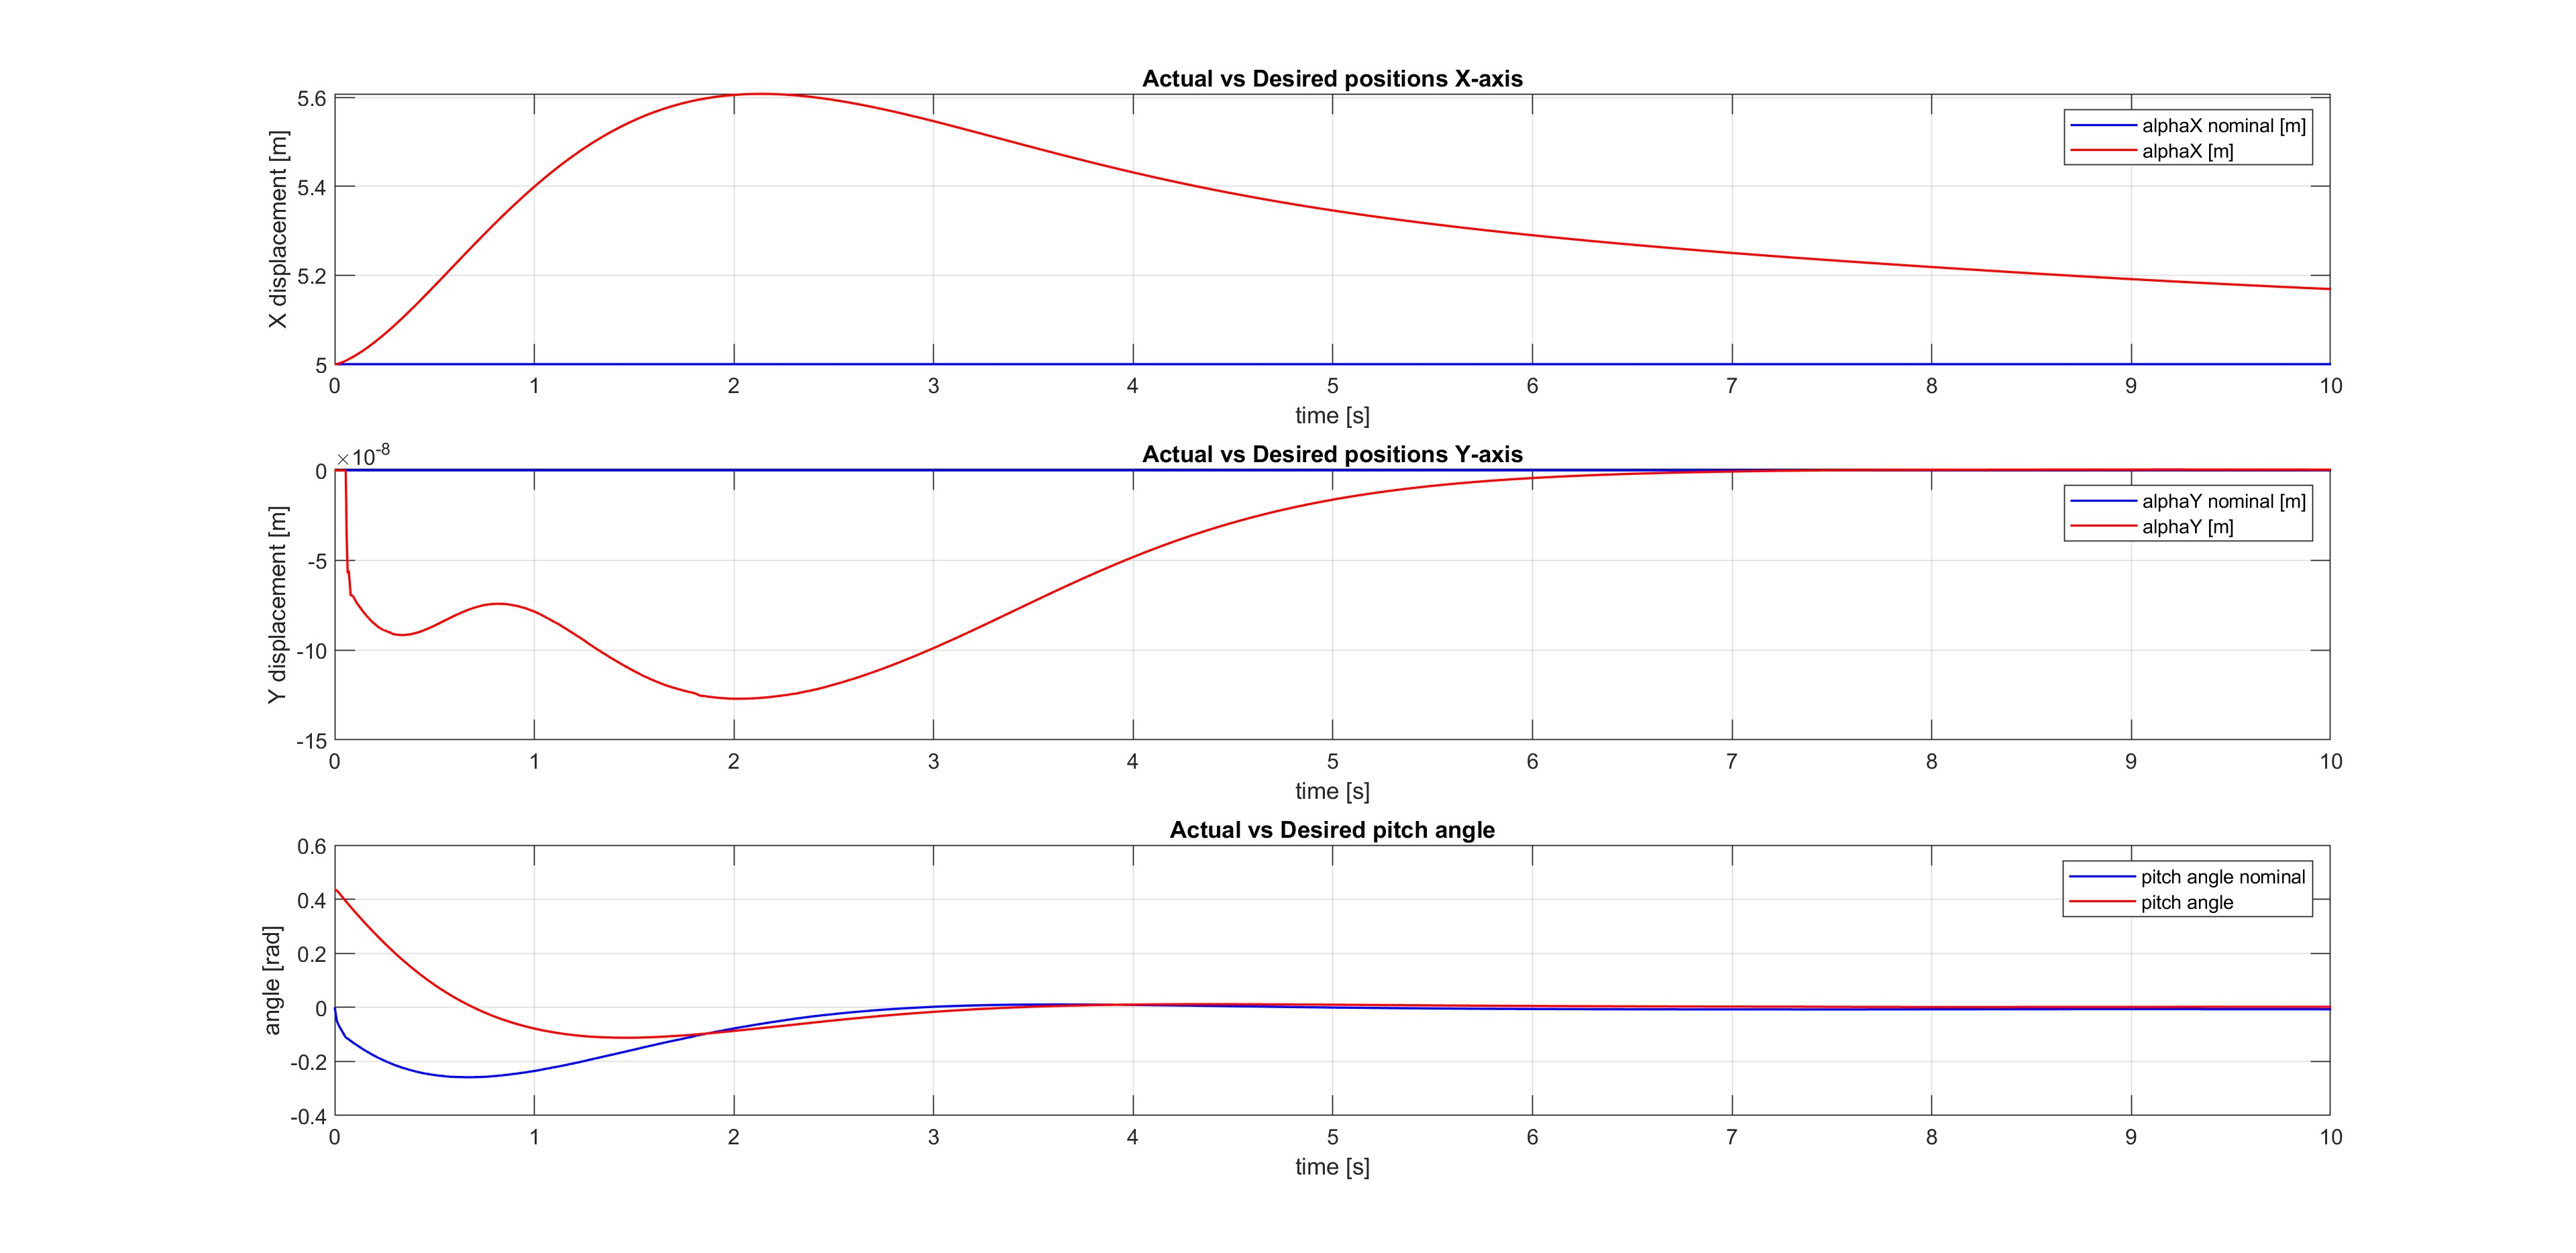
\includegraphics[width=1\linewidth]{Images/Robustness analysis/Unloaded/Swing-Up/Position_error.jpg}
    \caption{Swing-up position error with disturbances in the unloaded case.}
    \label{fig:Swing-up position error with disturbances in the unloaded case}
\end{figure}

\begin{figure}
    \centering
    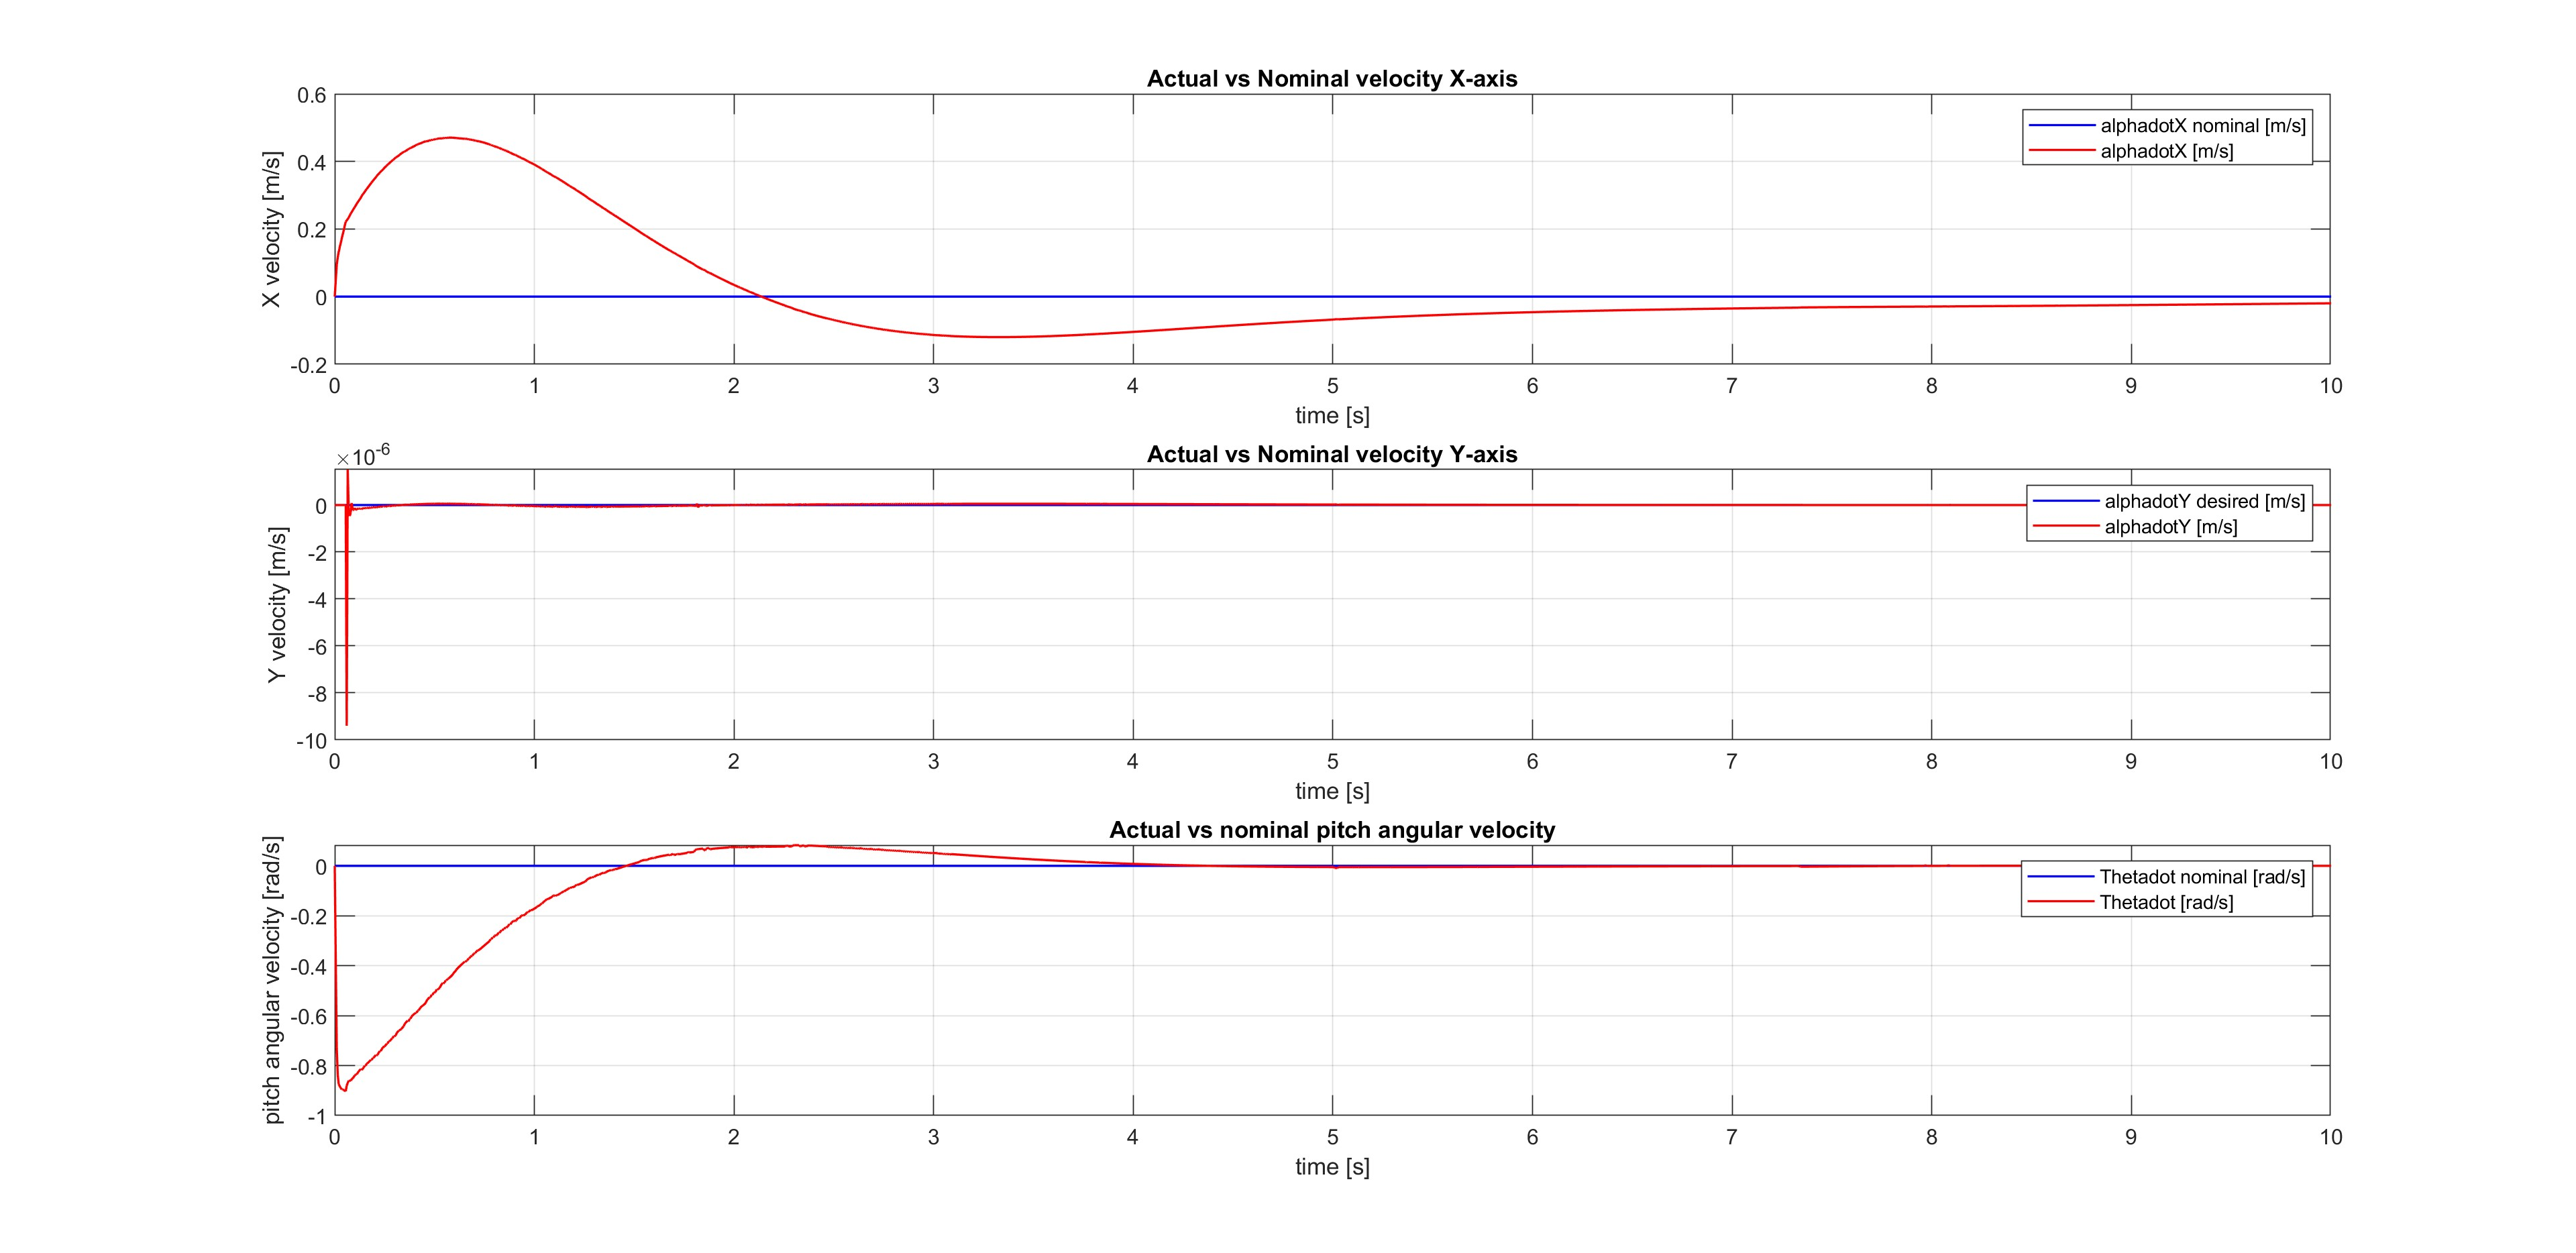
\includegraphics[width=1\linewidth]{Images/Robustness analysis/Unloaded/Swing-Up/Velocity_error.jpg}
    \caption{Swing-up velocity error with disturbances in the unloaded case.}
    \label{fig:Swing-up velocity error with disturbances in the unloaded case}
\end{figure}

Figures \ref{fig:Swing-up position error with disturbances in the unloaded case} and \ref{fig:Swing-up velocity error with disturbances in the unloaded case}, show the nominal and actual trajectories in position and velocity respectively for the unloaded condition, and it can be noticed how, after the transient, the actual trajectories approach the nominal ones.

Figure \ref{fig:Swing-up slipping velocity with disturbances in the unloaded case} instead shows in red the slipping velocity between the wheels and the terrain, and in green the solver status which is defined as follows: 

\begin{itemize}
    \item 1 = Solved
    \item 2 = Solved with higher tolerance
    \item -2 = maximum number of iterations reached
\end{itemize}

\begin{figure}
    \centering
    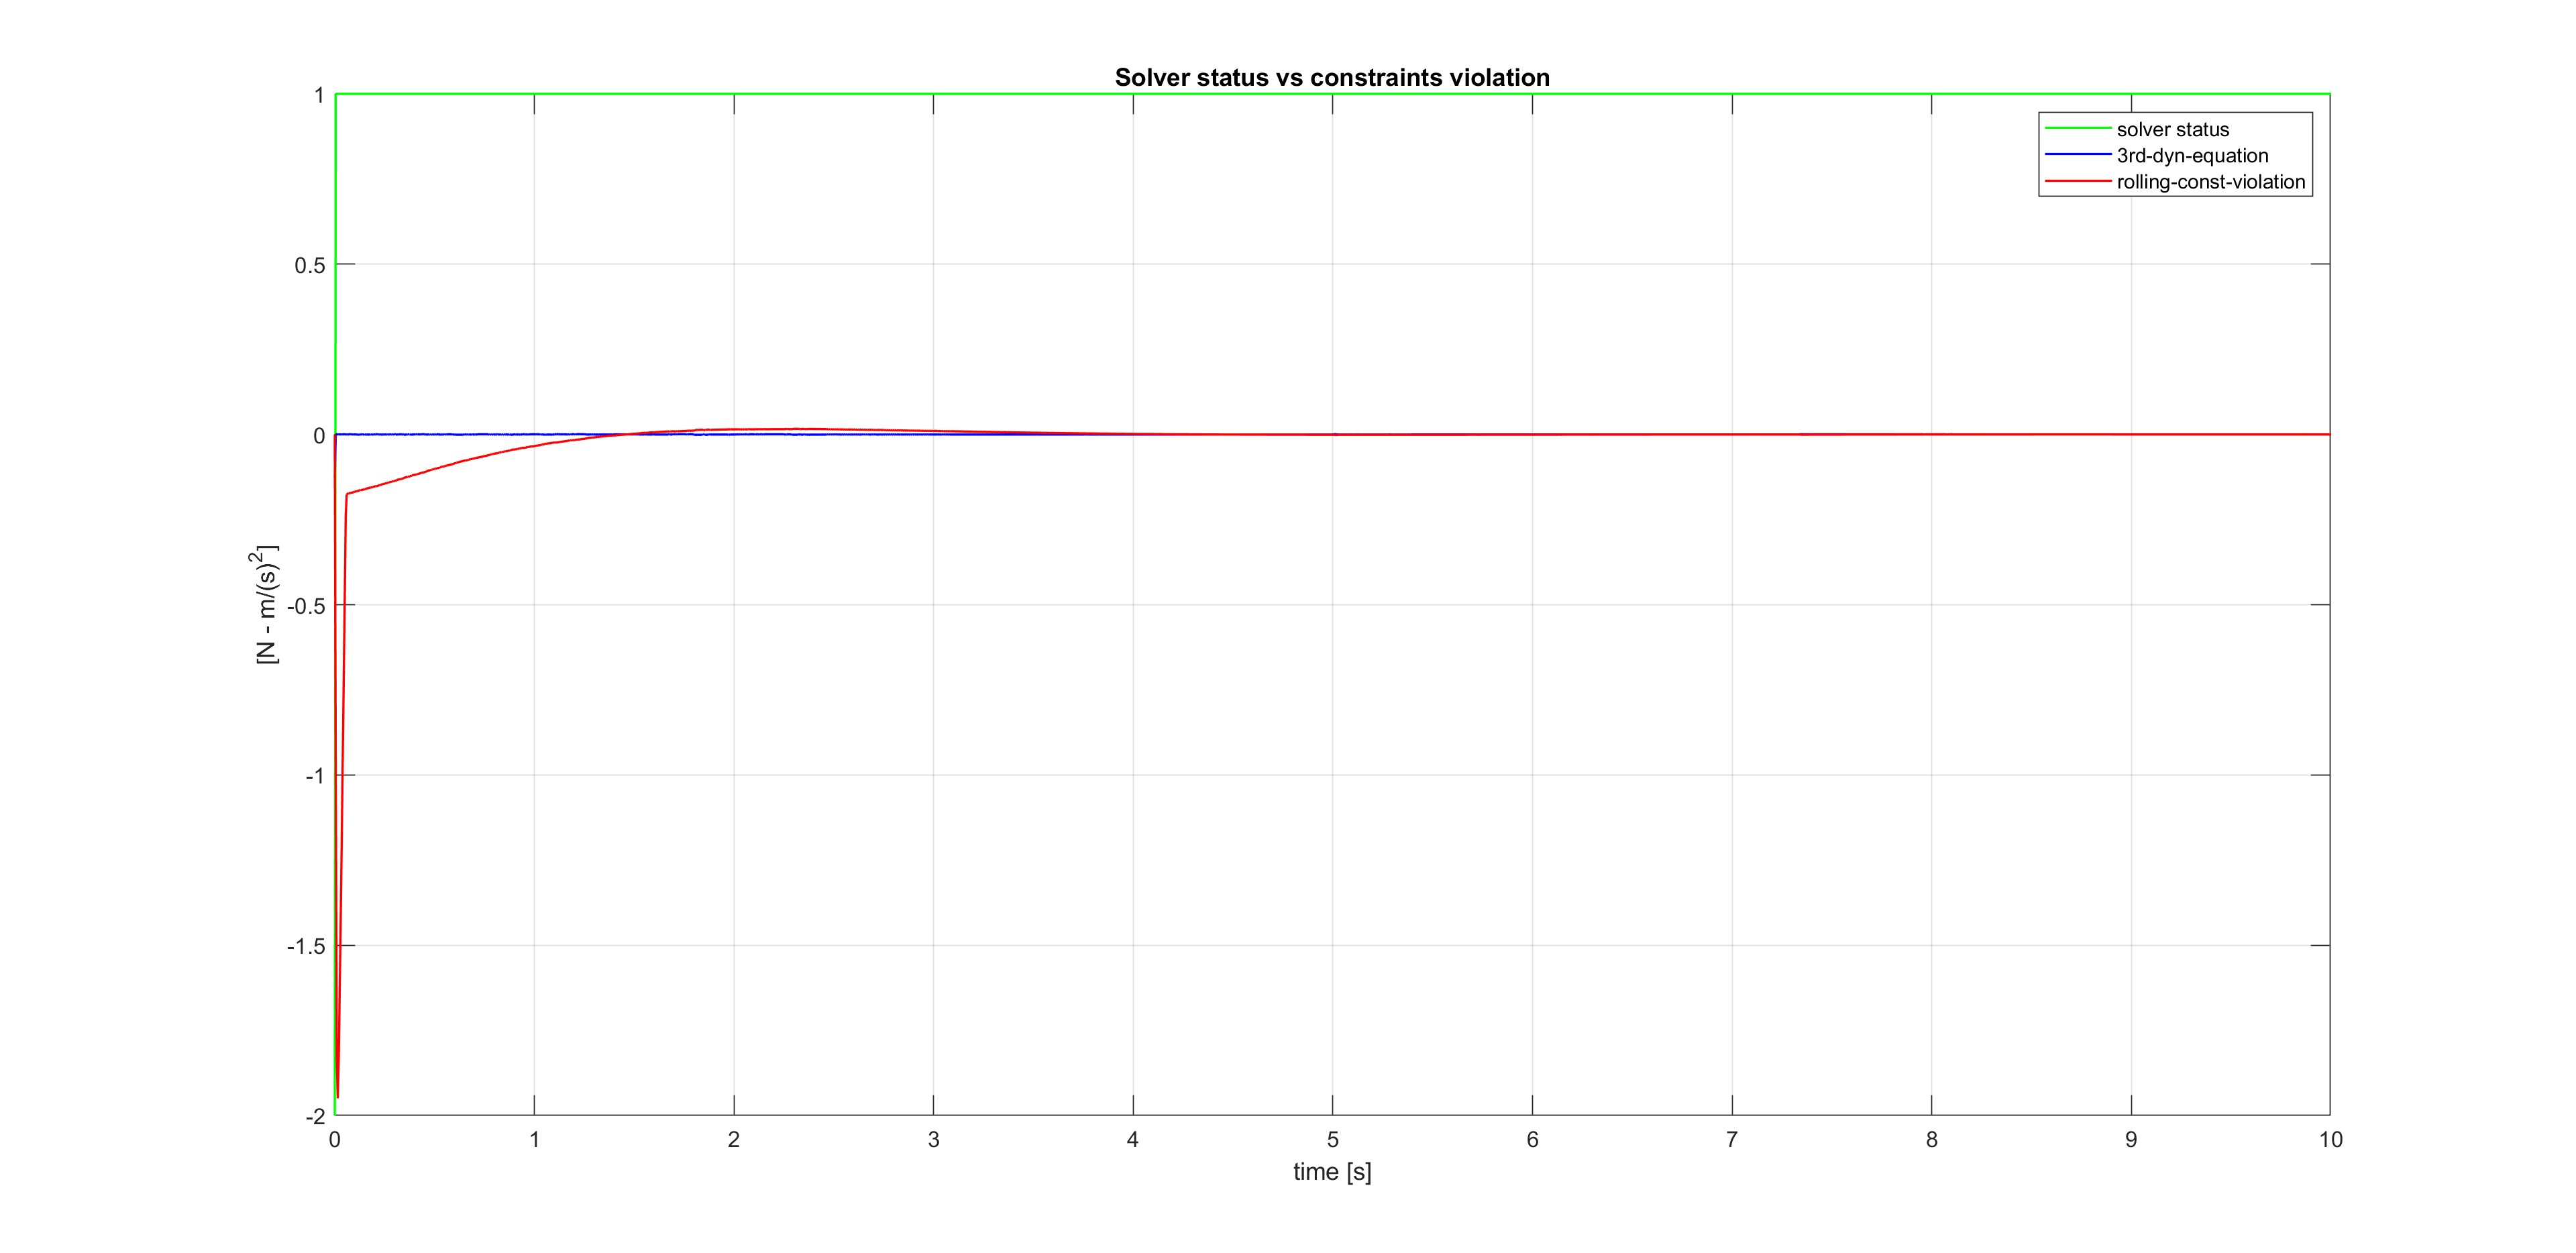
\includegraphics[width=1\linewidth]{Images/Robustness analysis/Unloaded/Swing-Up/Slipping_velocity.jpg}
    \caption{Swing-up slipping velocity with disturbances in the unloaded case.}
    \label{fig:Swing-up slipping velocity with disturbances in the unloaded case}
\end{figure}

\subsection{Swing-up in the case of half load}
\label{subsec:Swing-up in the case of half load}

\begin{figure}
    \centering
    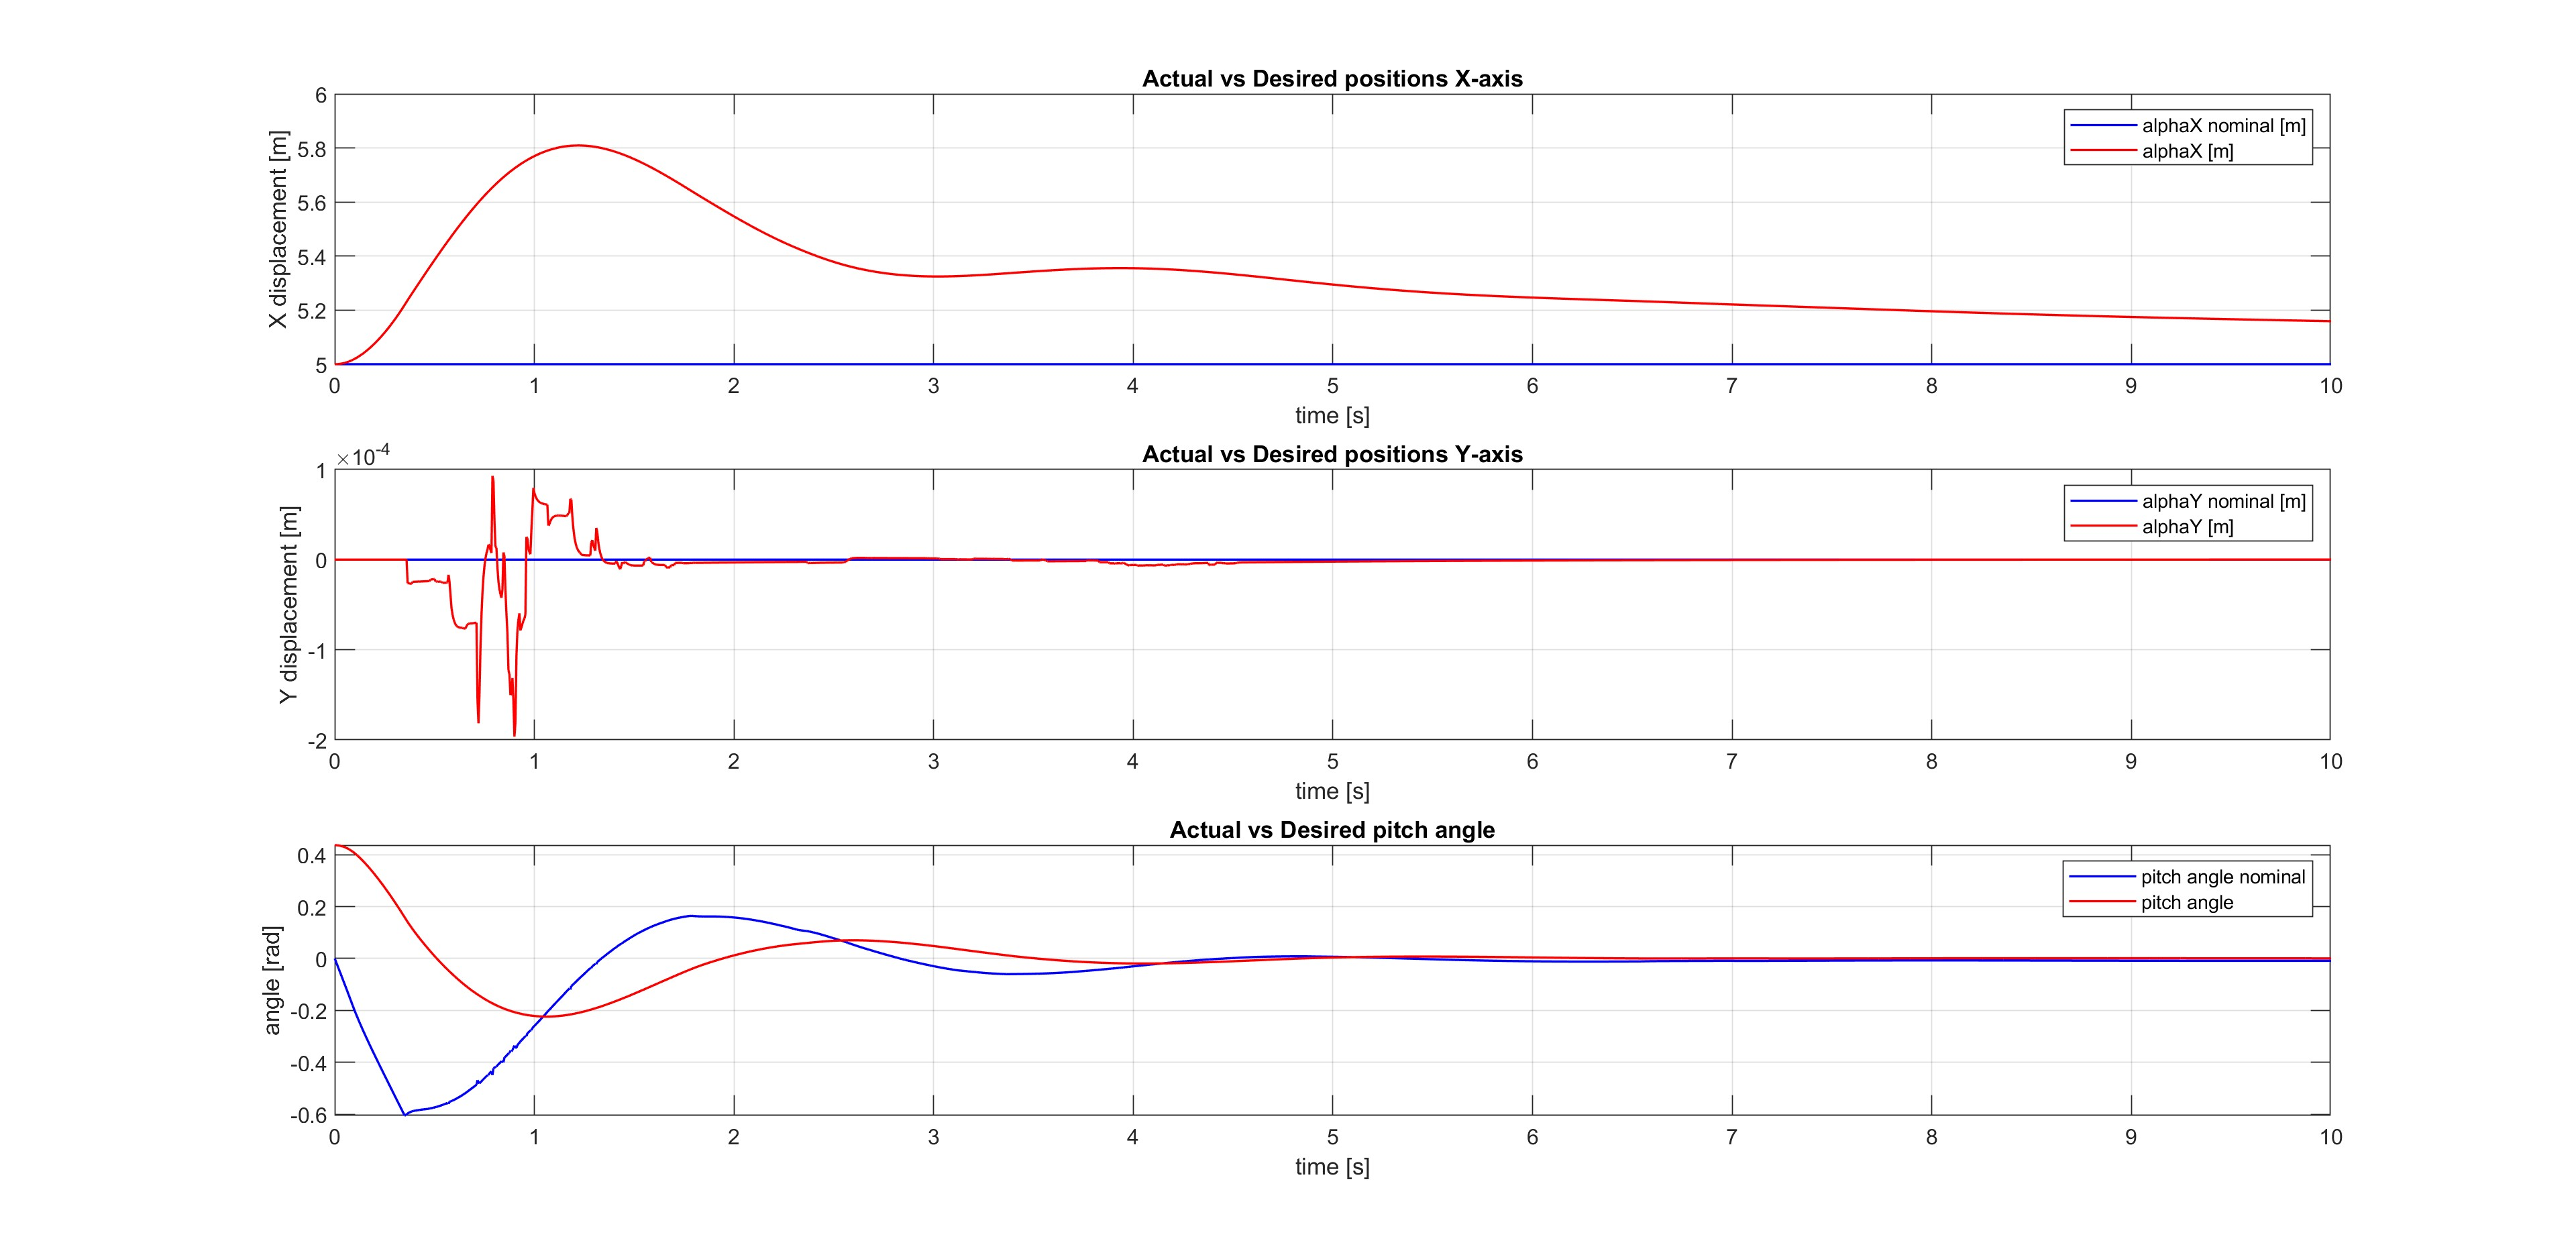
\includegraphics[width=1\linewidth]{Images/Robustness analysis/intermediate load/Swing-Up/Position_error.jpg}
    \caption{Swing-up position error with disturbances in the case of half load.}
    \label{fig:Swing-up position error with disturbances in the case of half load}
\end{figure}

\begin{figure}
    \centering
    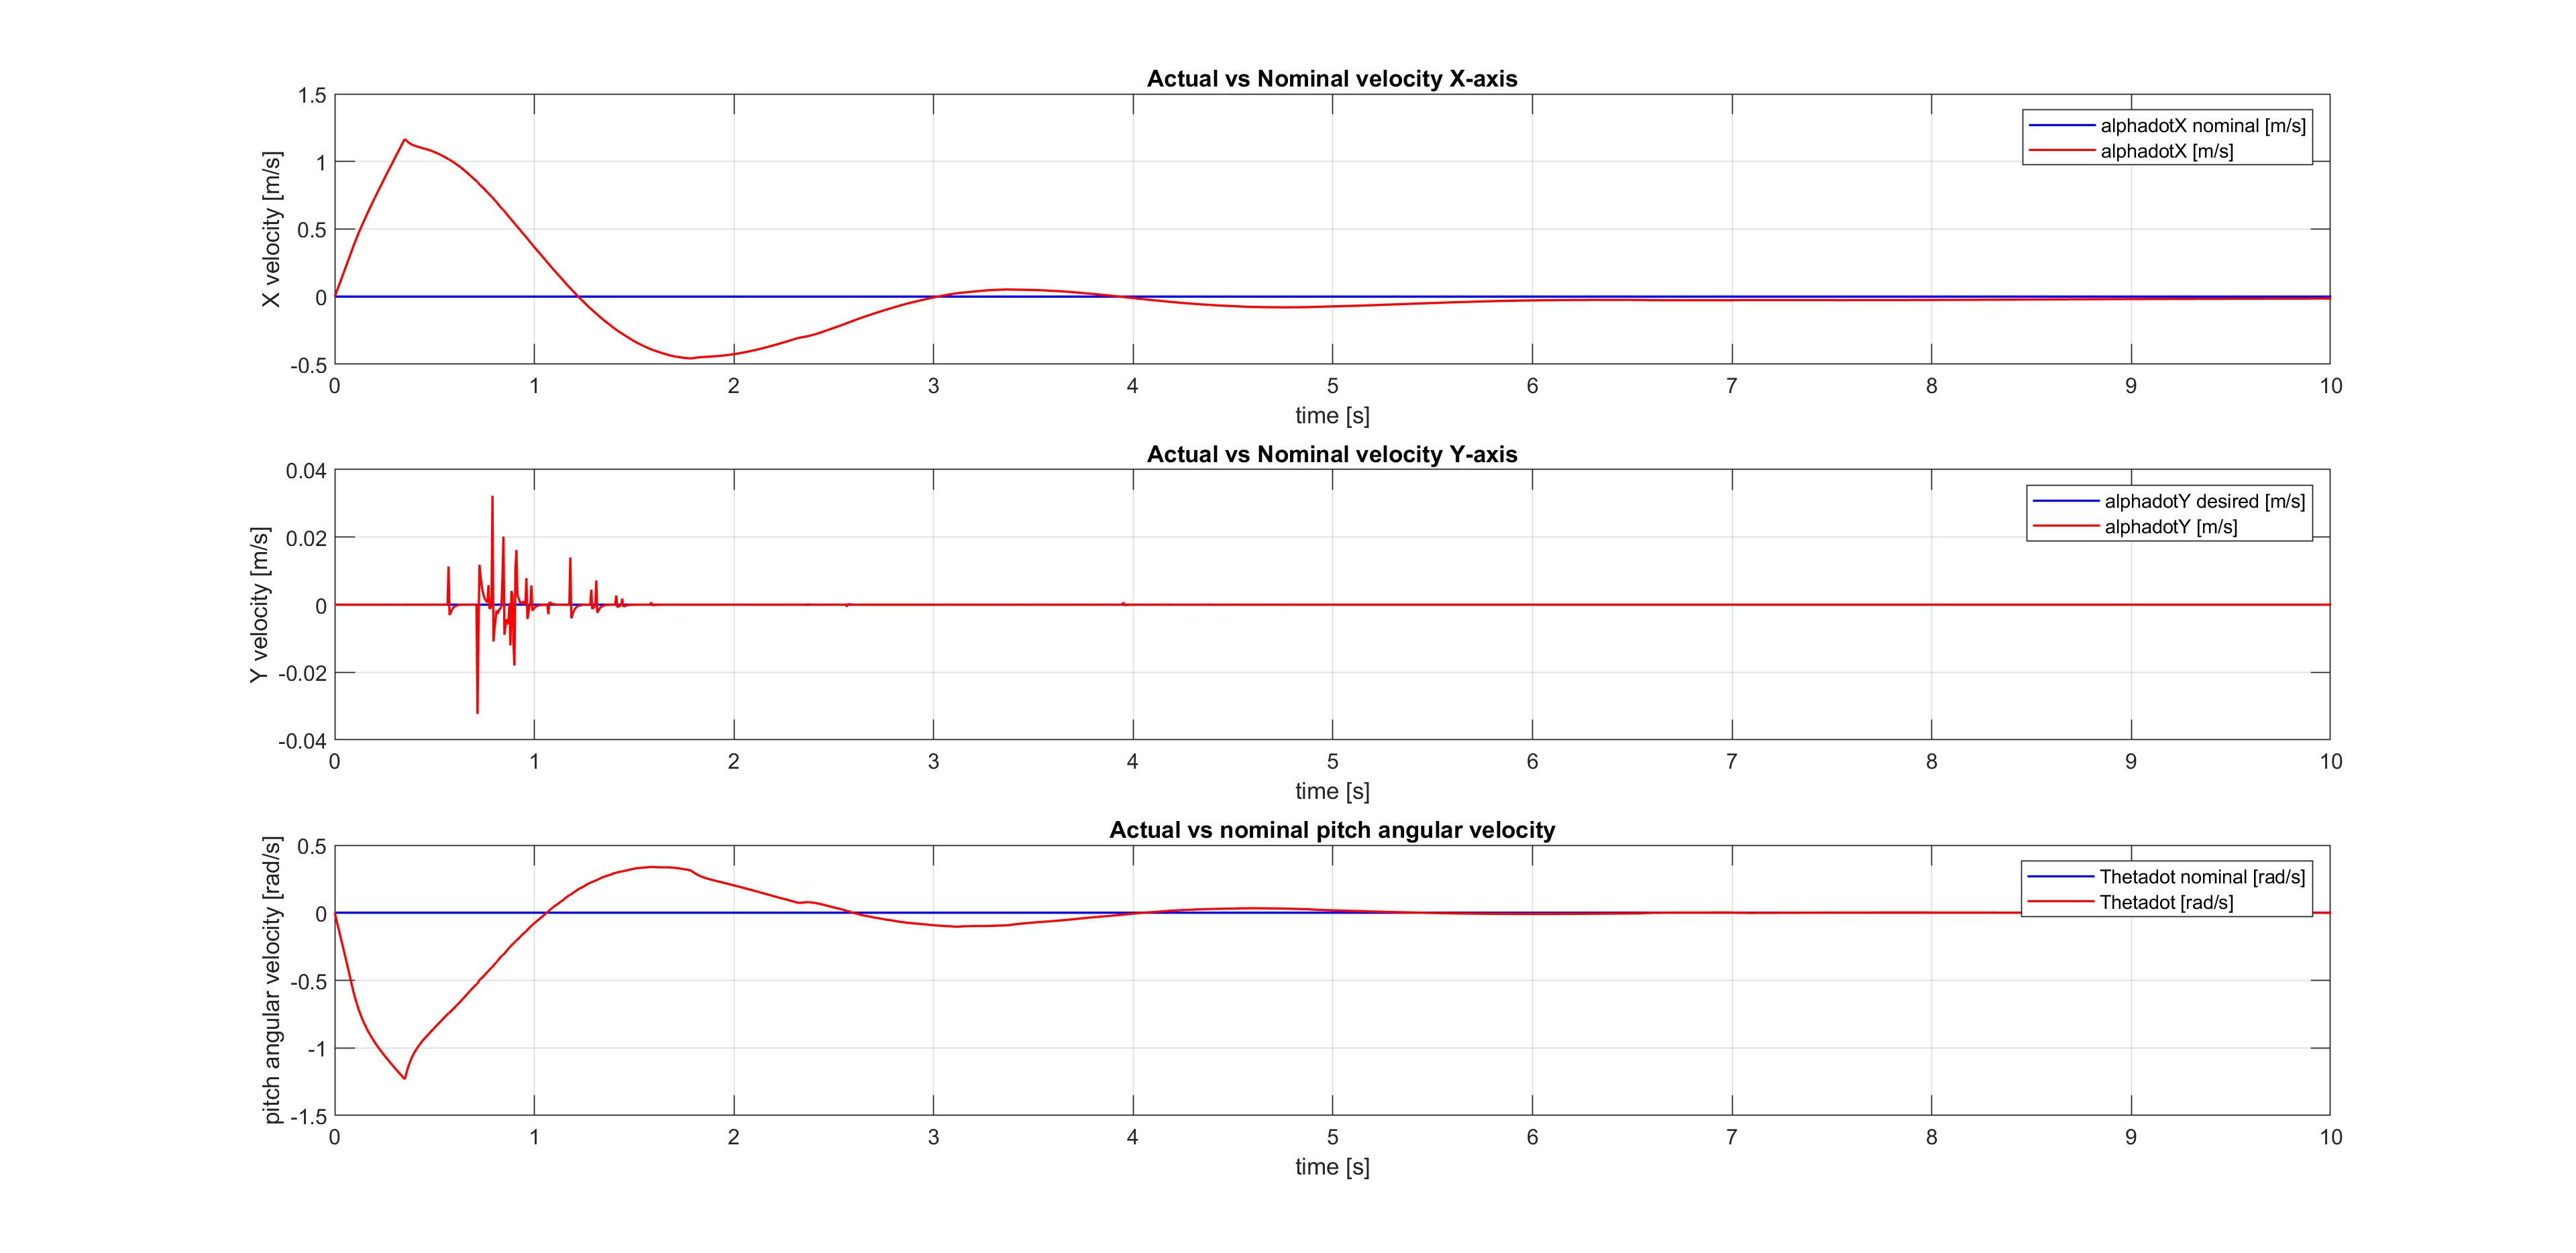
\includegraphics[width=1\linewidth]{Images/Robustness analysis/intermediate load/Swing-Up/Velocity_error.jpg}
    \caption{Swing-up velocity error with disturbances in the case of half load.}
    \label{fig:Swing-up velocity error with disturbances in the case of half load}
\end{figure}

Figures \ref{fig:Swing-up position error with disturbances in the case of half load} and \ref{fig:Swing-up velocity error with disturbances in the case of half load}, show the nominal and actual trajectories in position and velocity respectively for the condition of half load, and also in this case, after the transient, the actual trajectories approach the nominal ones.
In this situation there is a perfect match regarding the controller model and the simulator one, apart for the friction coefficient.

\begin{figure}
    \centering
    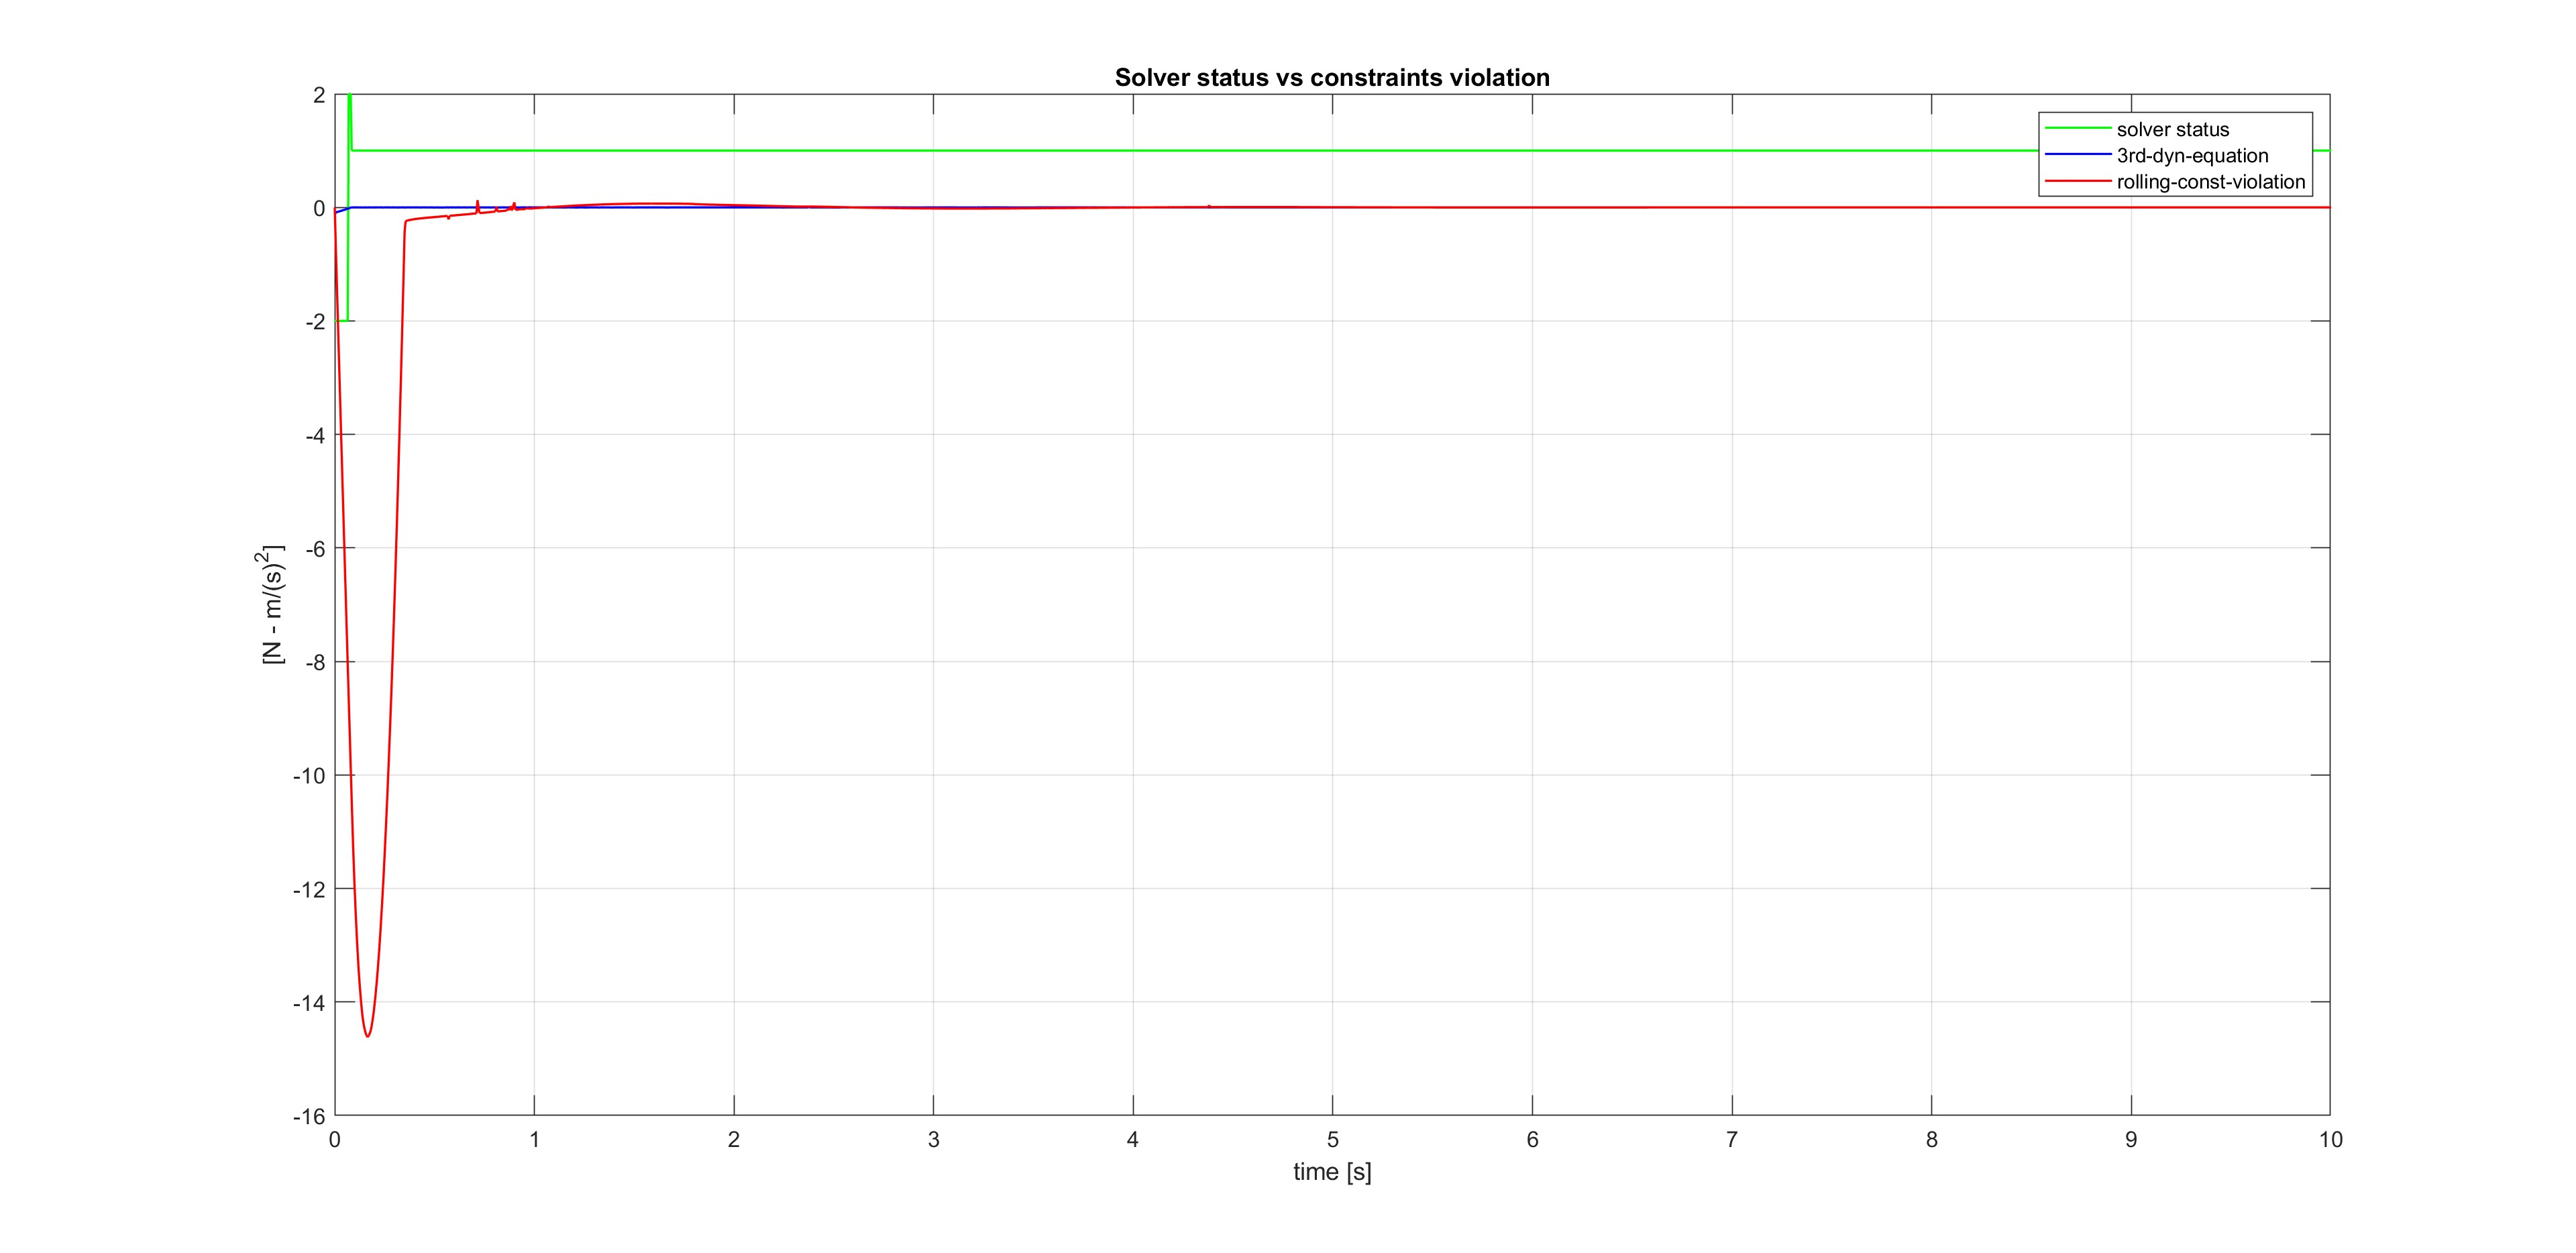
\includegraphics[width=1\linewidth]{Images/Robustness analysis/intermediate load/Swing-Up/Slipping_velocity.jpg}
    \caption{Swing-up slipping velocity with disturbances in the case of half load.}
    \label{fig:Swing-up slipping velocity with disturbances in the case of half load}
\end{figure}

In Figure \ref{fig:Swing-up slipping velocity with disturbances in the case of half load} is represented in red the slipping velocity, and in green the solver status.

\subsection{Swing-up in the case of maximum load}
\label{subsec:Swing-up in the case of maximum load}

\begin{figure}
    \centering
    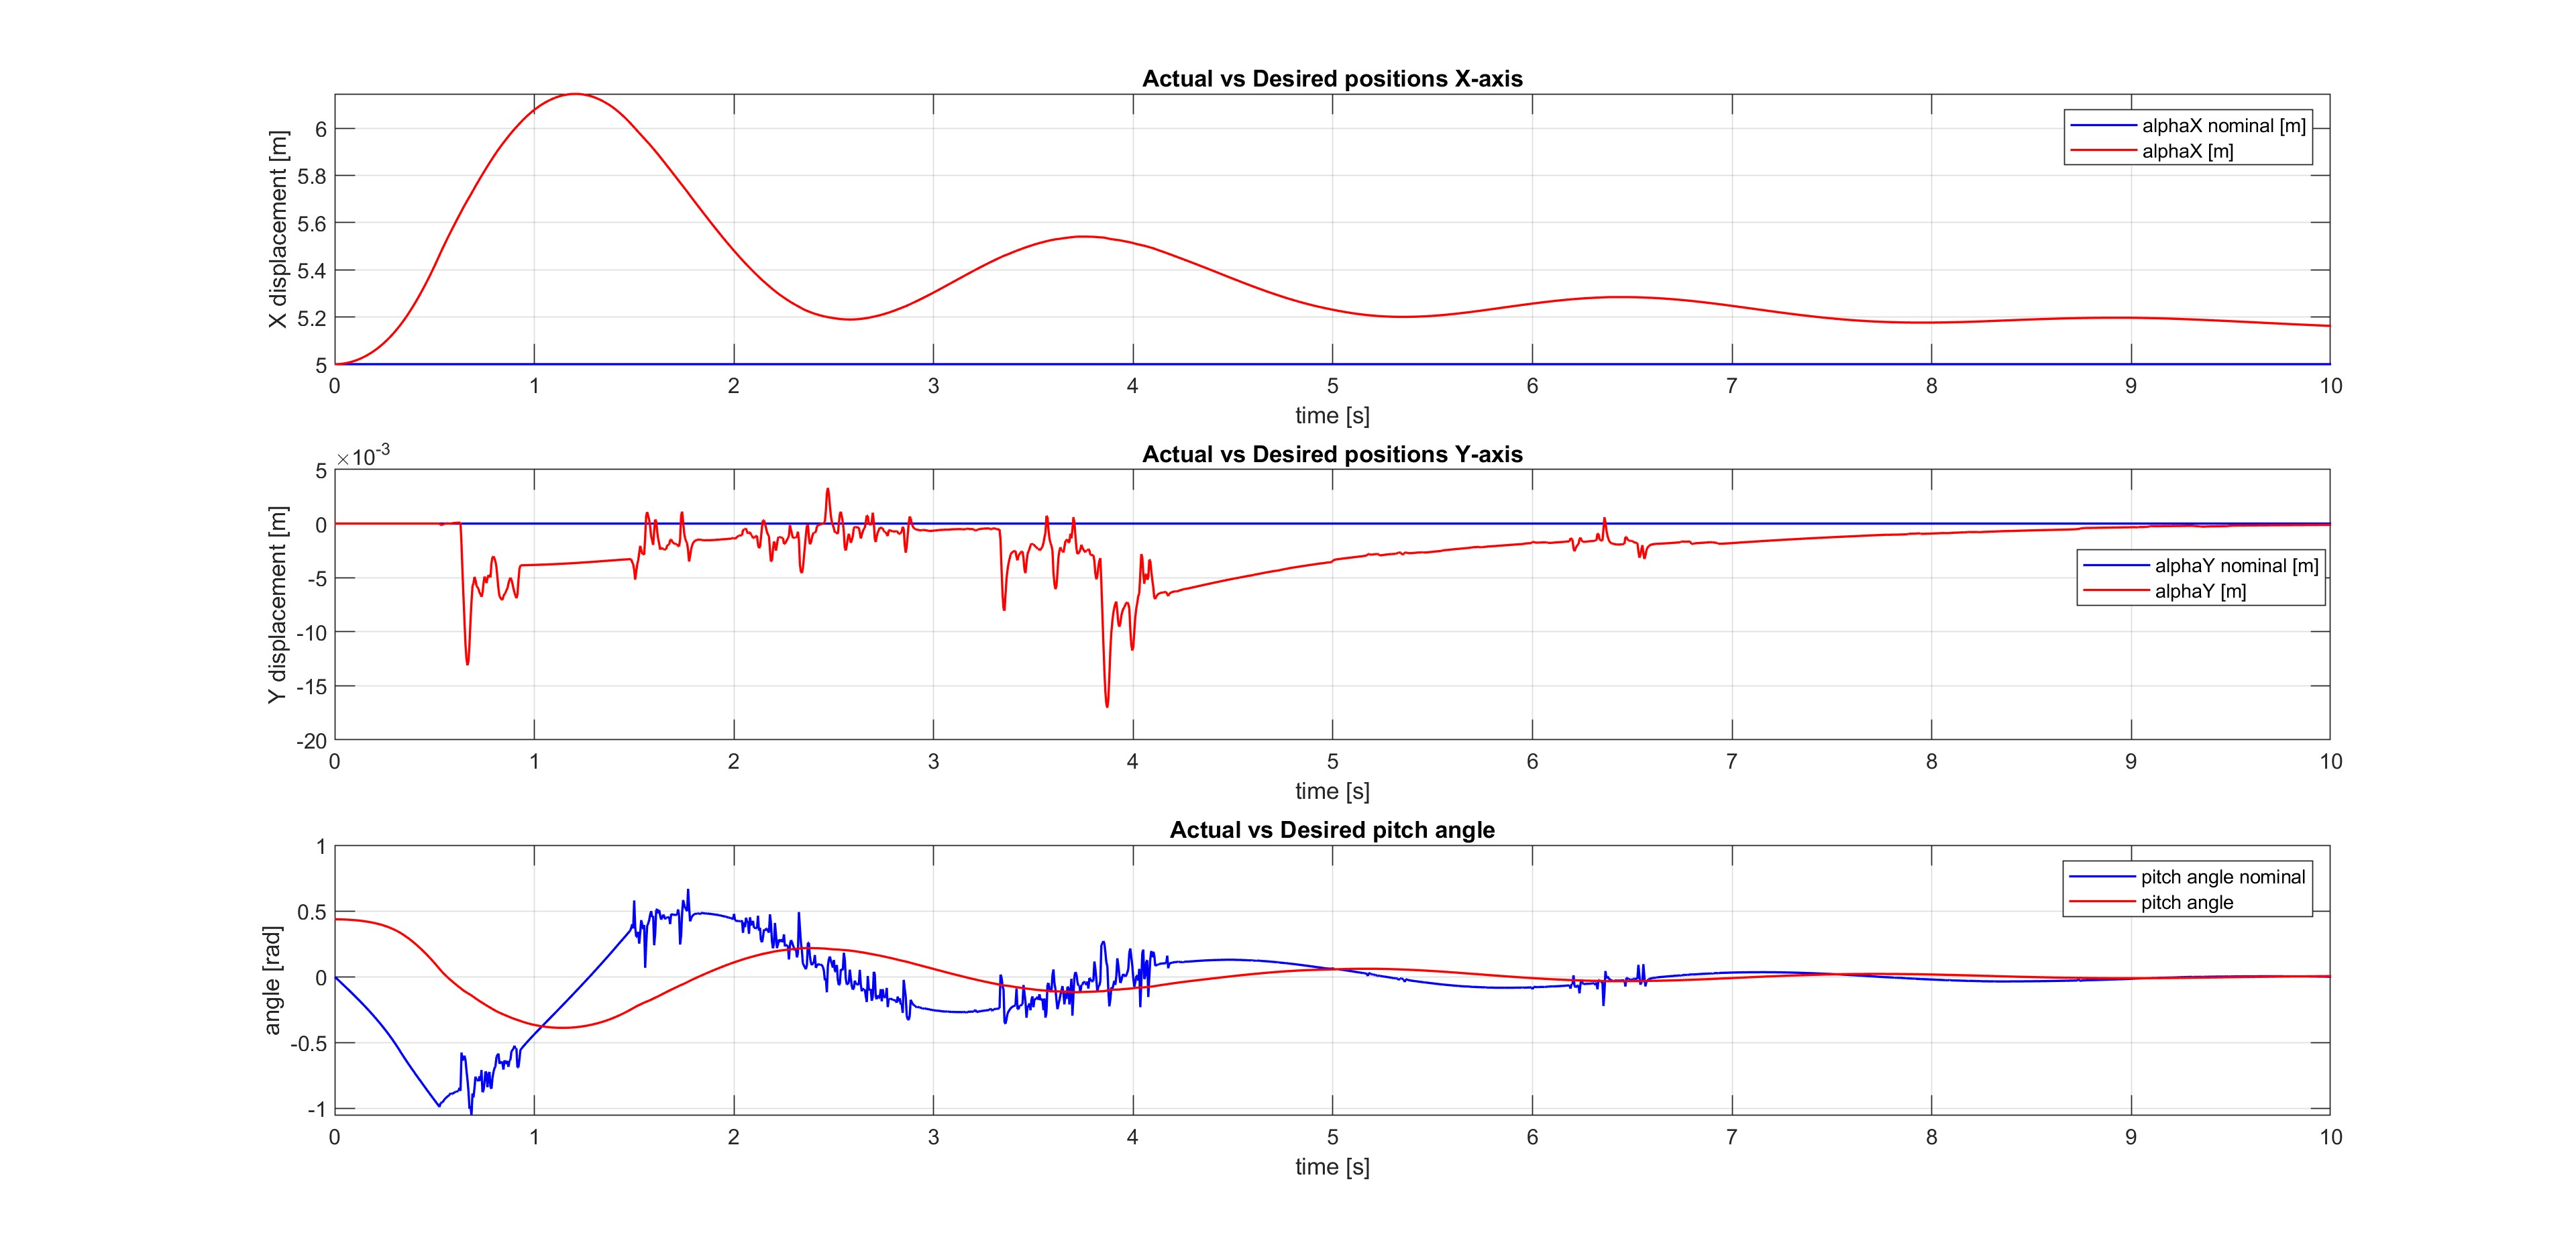
\includegraphics[width=1\linewidth]{Images/Robustness analysis/maximum load/Swing-Up/Position_error.jpg}
    \caption{Swing-up position error with disturbances in the case of maximum load.}
    \label{fig:Swing-up position error with disturbances in the case of maximum load}
\end{figure}

\begin{figure}
    \centering
    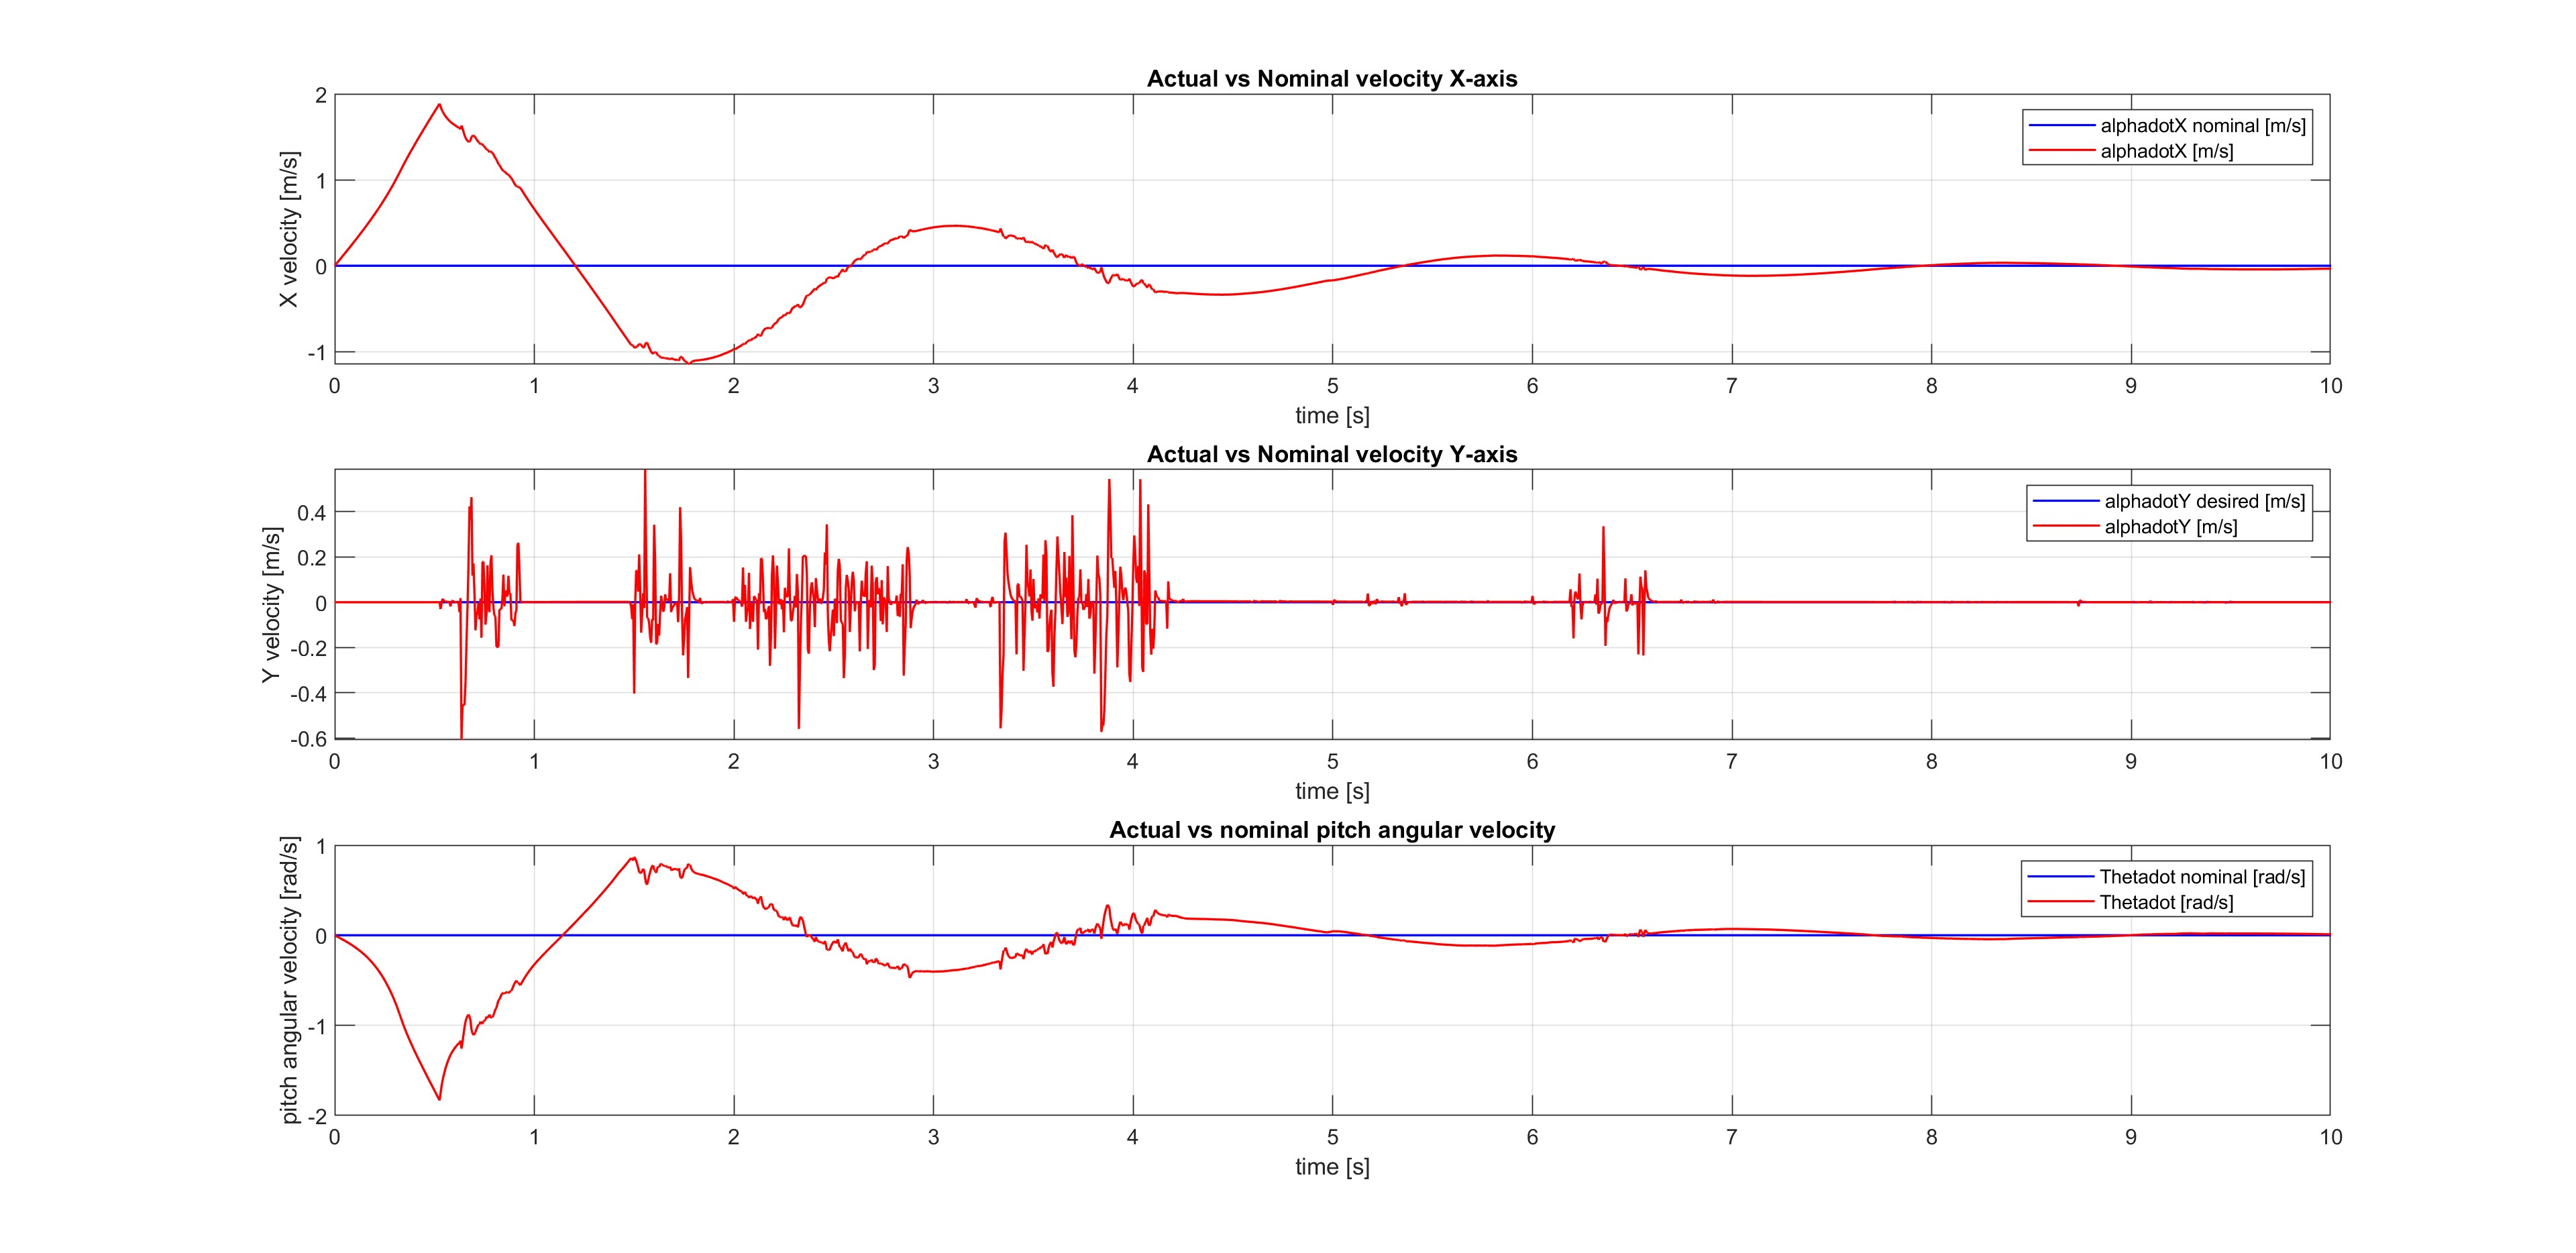
\includegraphics[width=1\linewidth]{Images/Robustness analysis/maximum load/Swing-Up/Velocity_error.jpg}
    \caption{Swing-up velocity error with disturbances in the case of maximum load.}
    \label{fig:Swing-up velocity error with disturbances in the case of maximum load}
\end{figure}

Figures \ref{fig:Swing-up position error with disturbances in the case of maximum load} and \ref{fig:Swing-up velocity error with disturbances in the case of maximum load}, show the nominal and actual trajectories in position and velocity respectively for the extreme condition of maximum load, and also in this case, the pitch angle $\theta$ is stabilized after 5 seconds.
This simulation represents the worse possible case, in the sense that the pitch starting angle is the maximum possible, the same holds for the load, and the friction coefficient is very low.   

\begin{figure}
    \centering
    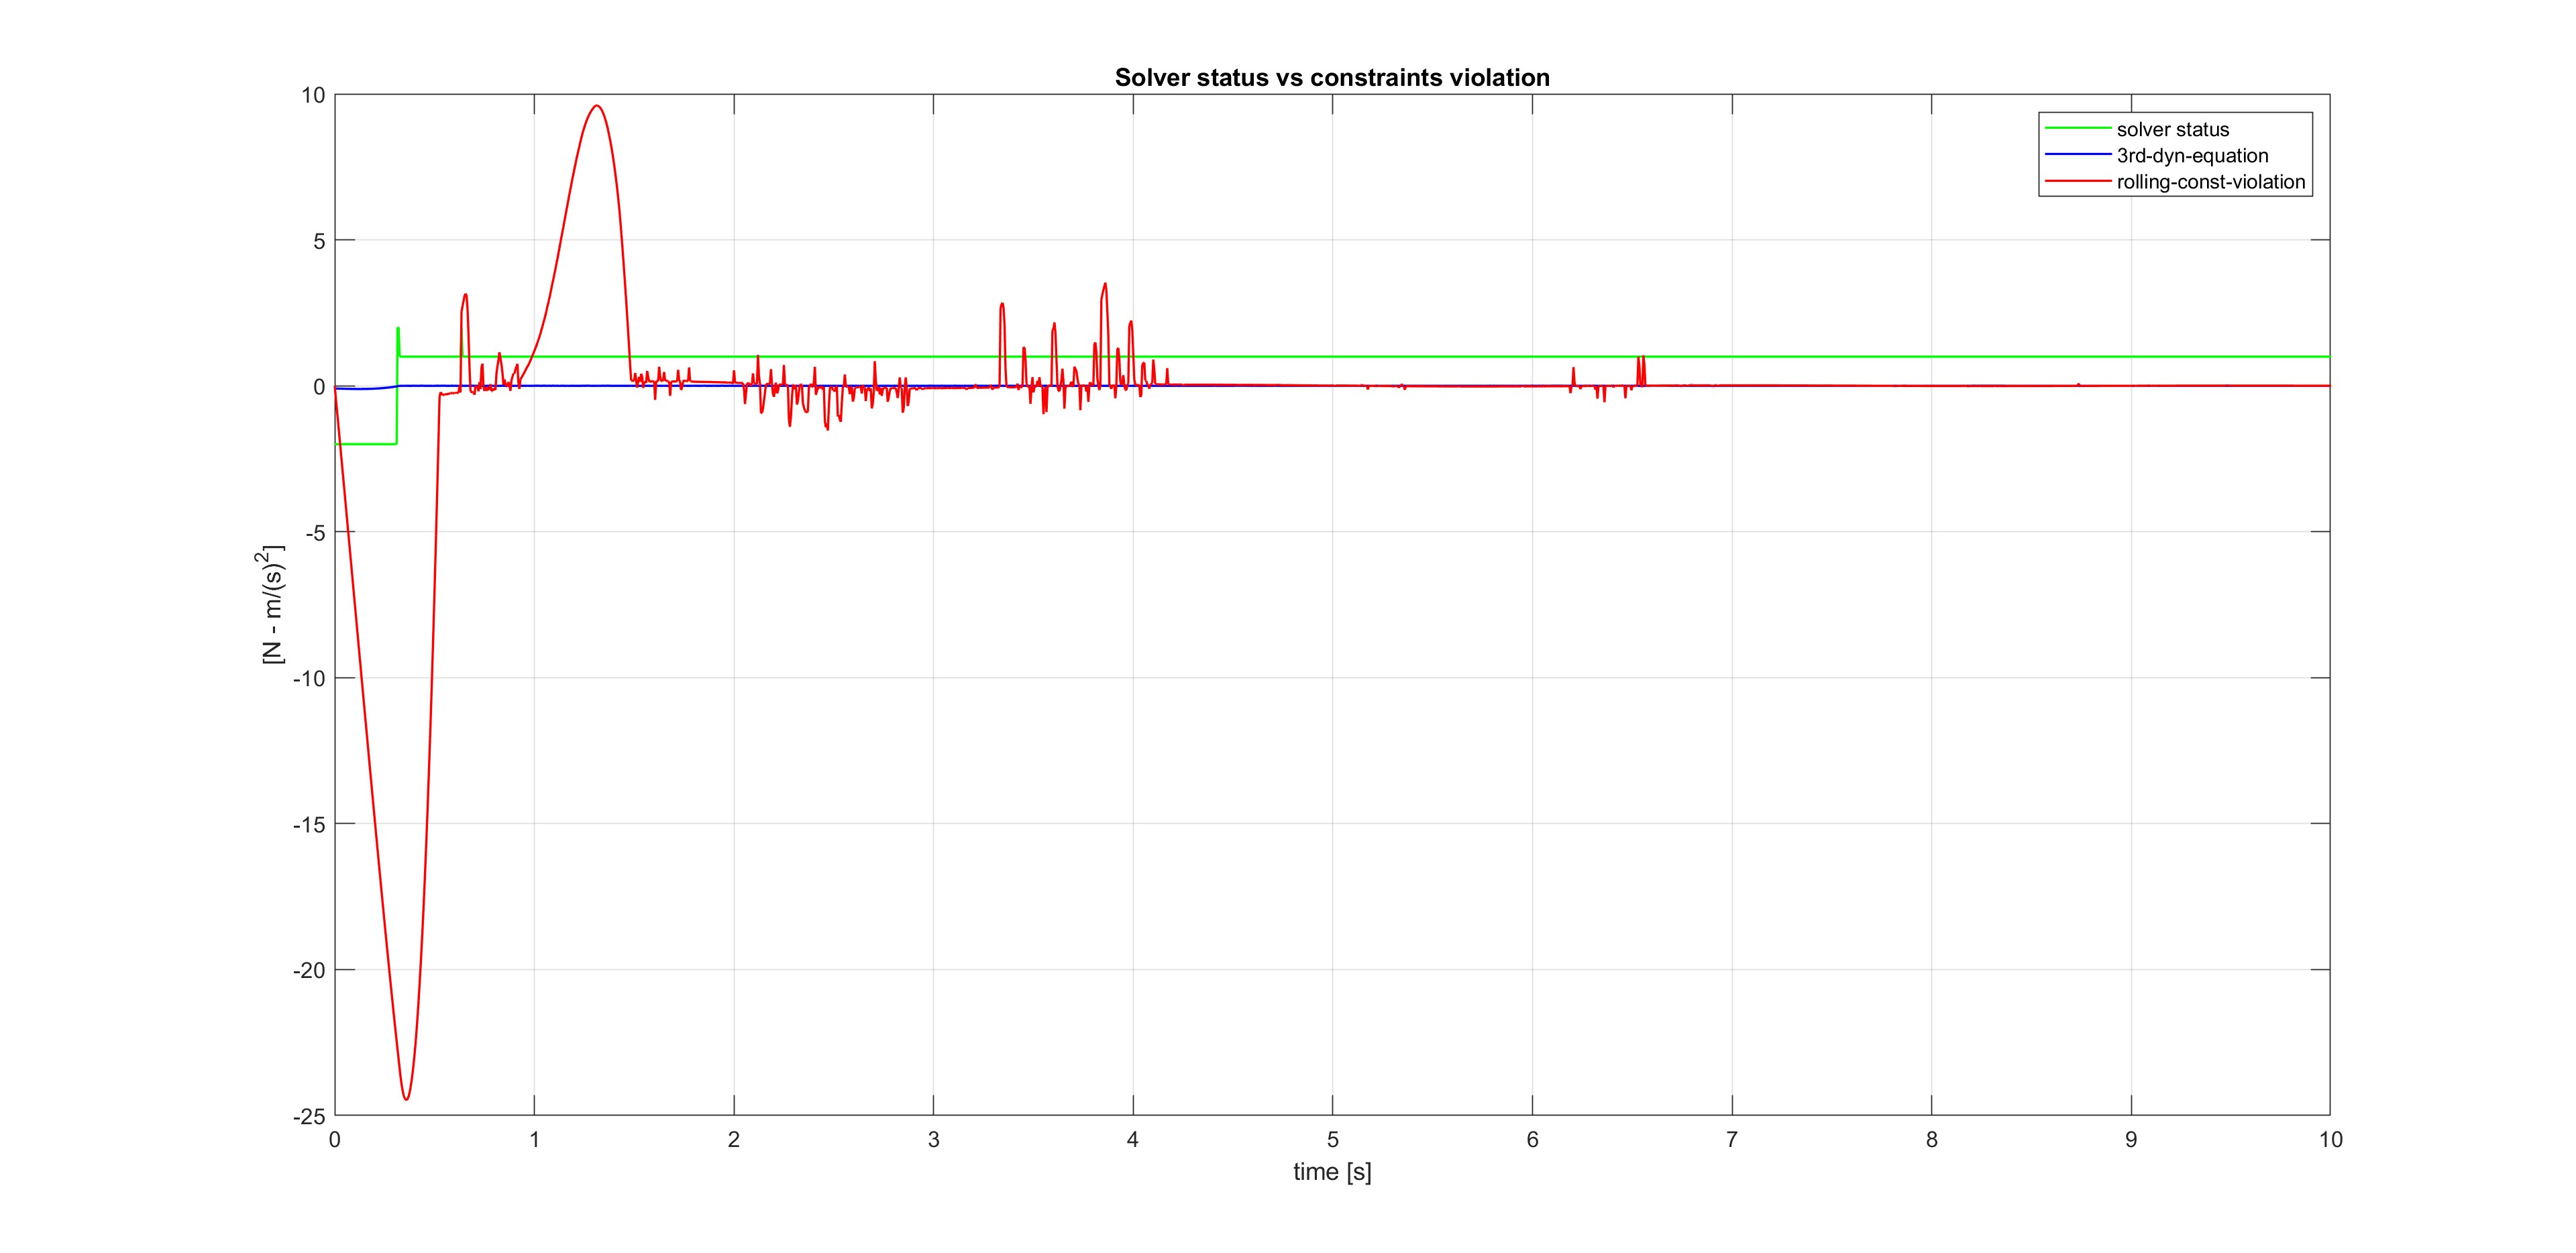
\includegraphics[width=1\linewidth]{Images/Robustness analysis/maximum load/Swing-Up/Slipping_velocity.jpg}
    \caption{Swing-up slipping velocity with disturbances in the case of maximum load.}
    \label{fig:Swing-up slipping velocity with disturbances in the case of maximum load}
\end{figure}

From Figure \ref{fig:Swing-up slipping velocity with disturbances in the case of maximum load}, representing in red the slipping velocity and in green the solver status, it can be noticed that for the first 0.5 seconds, the solver status is -2 due to an initial slipping velocity significantly different from zero. 

\section{Sinusoidal Trajectory with model uncertainties}
\label{sec:Sinusoidal Trajectory with model uncertainties}

Here we directly test a general nominal trajectory in the plane x-y for all the three conditions mentioned in the prologue of this chapter.

\subsection{Sinusoidal Trajectory in the unloaded case}
\label{subsec:Sinusoidal Trajectory in the unloaded case}

Figures \ref{fig:Sinusoidal trajectory position error with disturbances in the unloaded case} and \ref{fig:Sinusoidal trajectory velocity error with disturbances in the unloaded case}, show the nominal and actual trajectories in position and velocity respectively for the unloaded condition, and it can be noticed how, after the transient, the actual trajectories approach the nominal ones.
Some overshoots appear in Figure \ref{fig:Sinusoidal trajectory velocity error with disturbances in the unloaded case} due to the discontinuous acceleration profile.


\begin{figure}
    \centering
    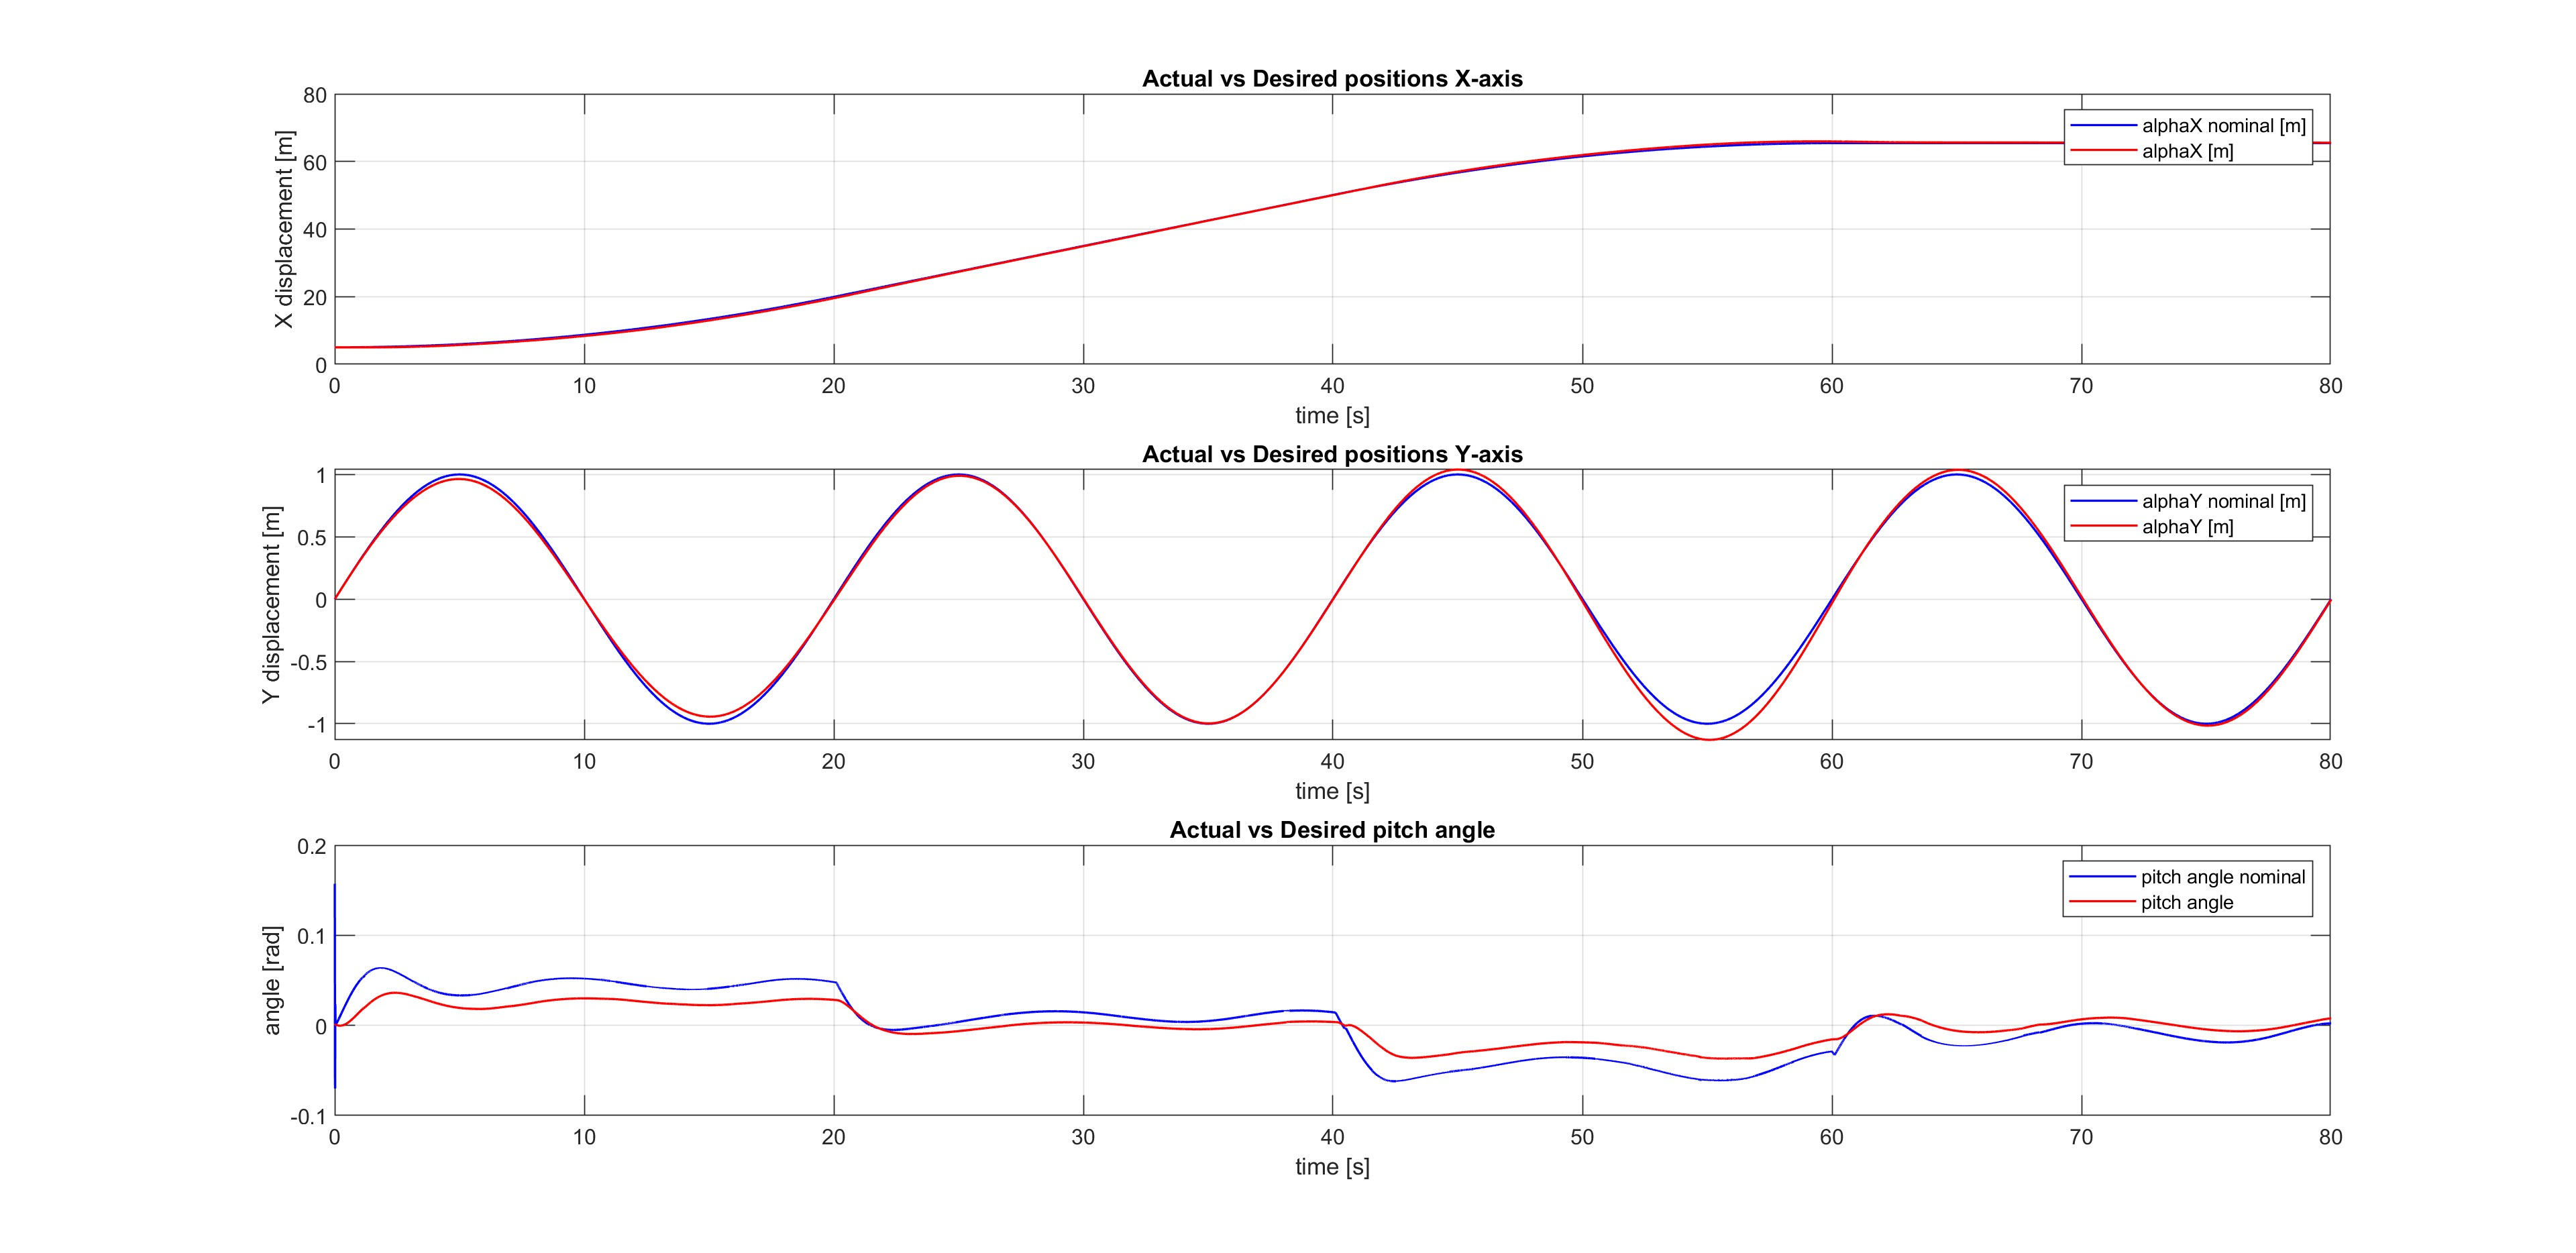
\includegraphics[width=1\linewidth]{Images/Robustness analysis/Unloaded/sinusoidal trajectory/Position_error.jpg}
    \caption{Sinusoidal trajectory position error with disturbances in the unloaded case.}
    \label{fig:Sinusoidal trajectory position error with disturbances in the unloaded case}
\end{figure}

\begin{figure}
    \centering
    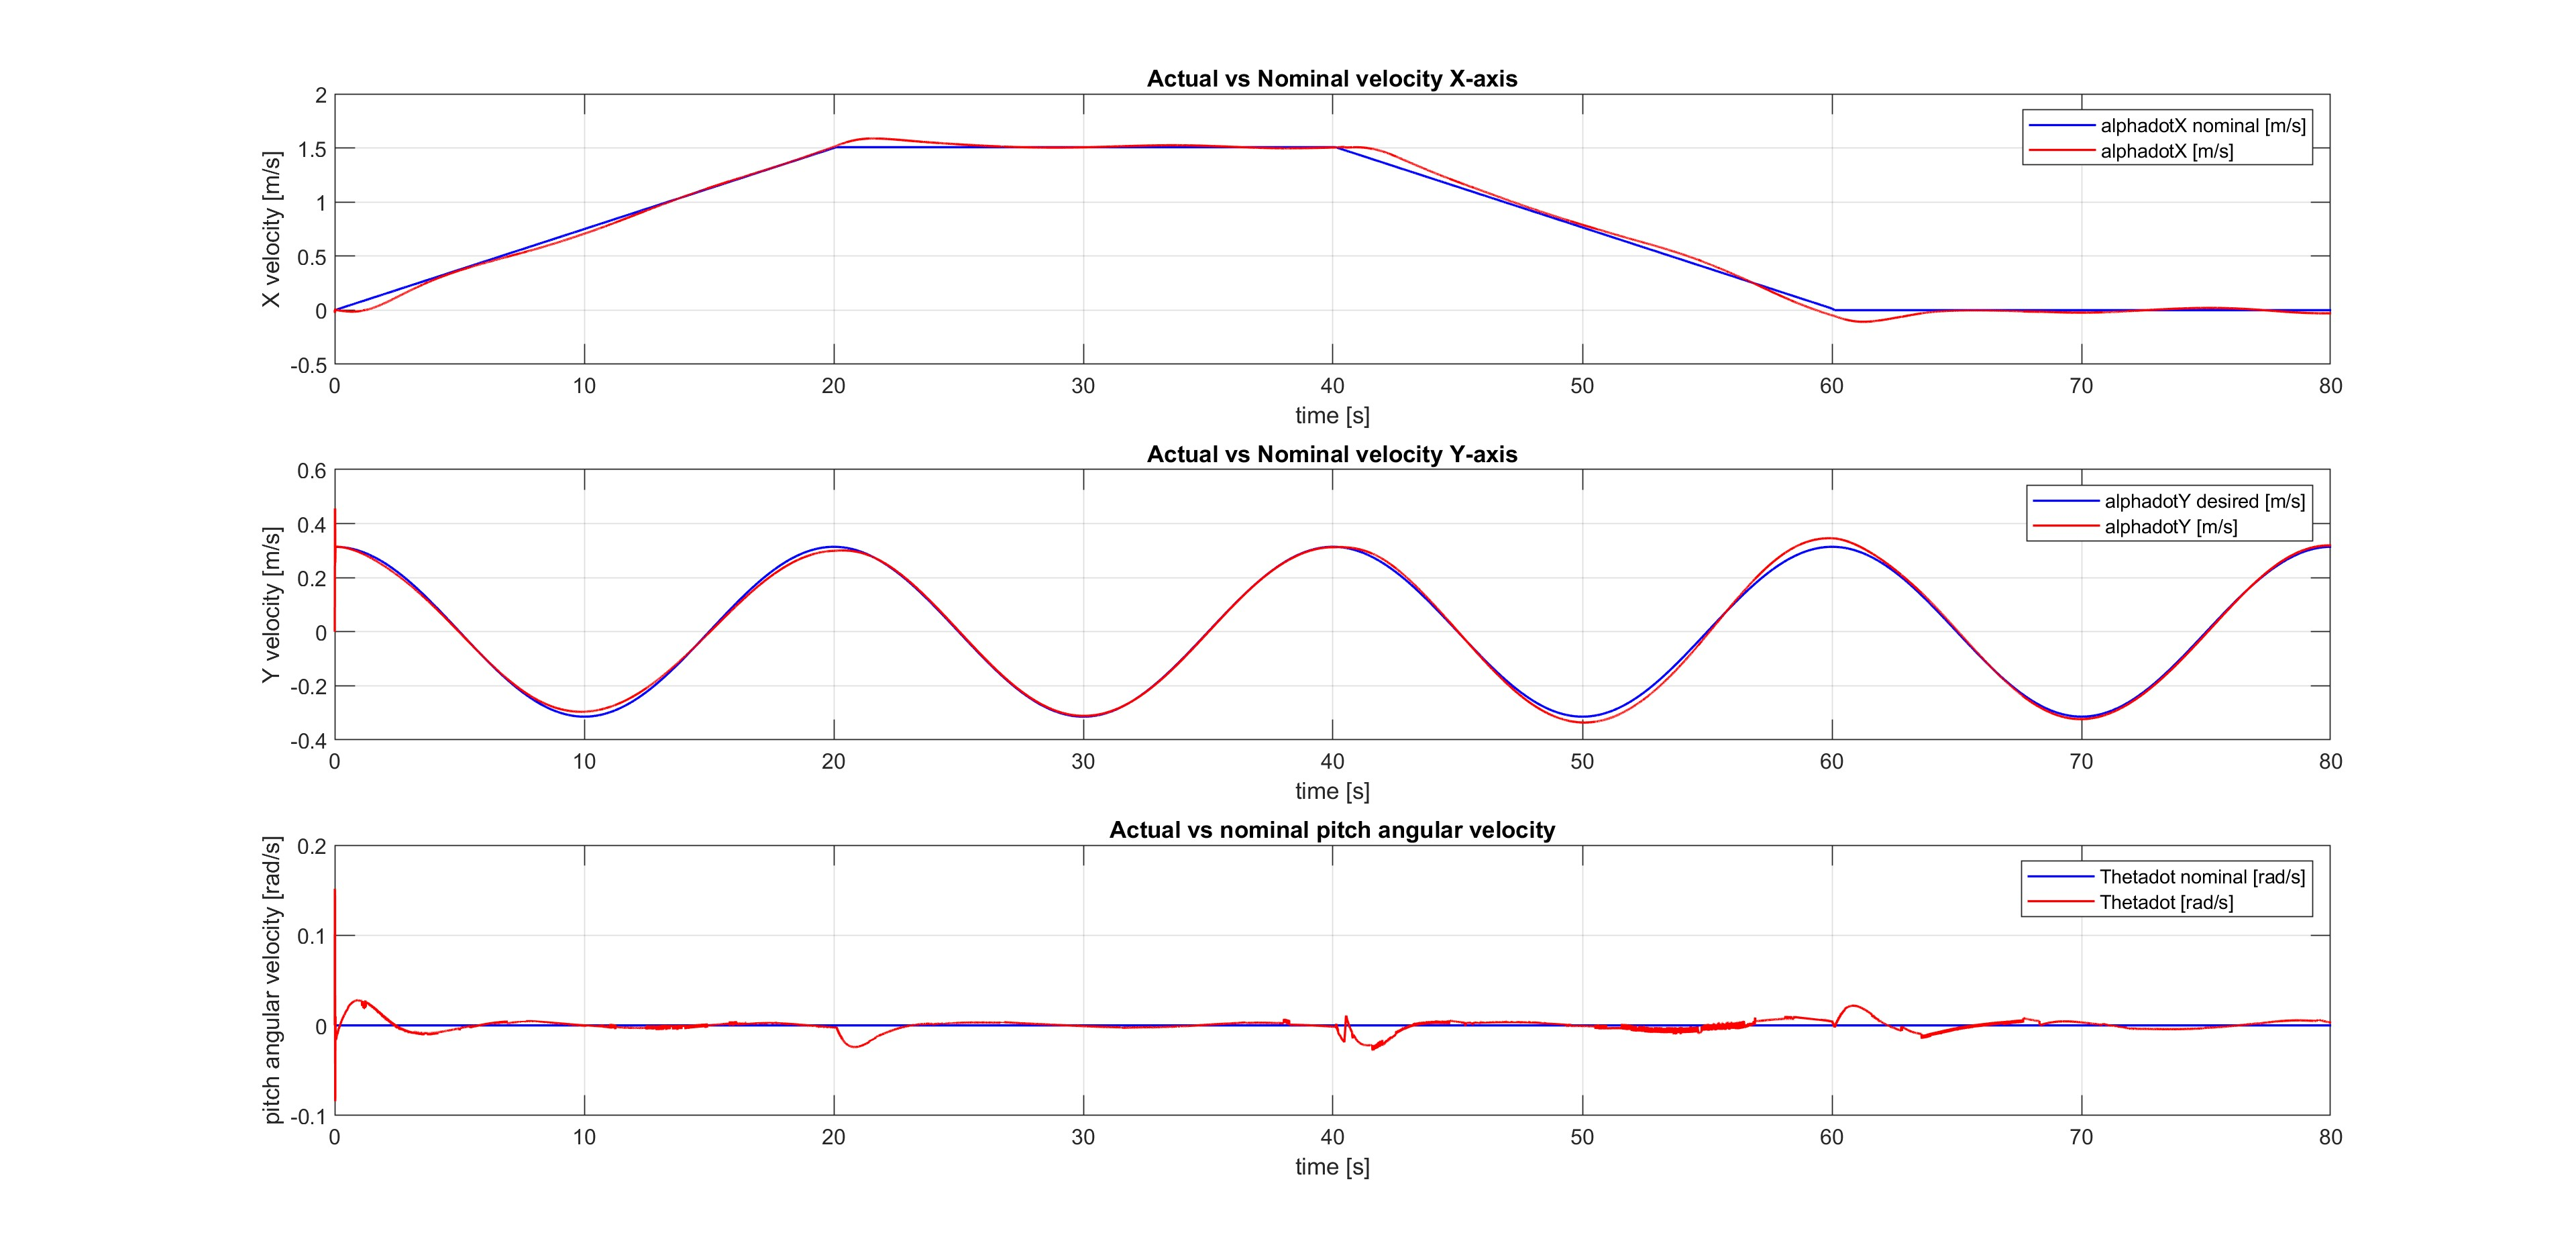
\includegraphics[width=1\linewidth]{Images/Robustness analysis/Unloaded/sinusoidal trajectory/Velocity_error.jpg}
    \caption{Sinusoidal trajectory velocity error with disturbances in the unloaded case.}
    \label{fig:Sinusoidal trajectory velocity error with disturbances in the unloaded case}
\end{figure}

Figure \ref{fig:Sinusoidal trajectory slipping velocity with disturbances in the unloaded case} instead shows in red the slipping velocity between the wheels and the terrain, and in green the solver status which is always =1.

\begin{figure}
    \centering
    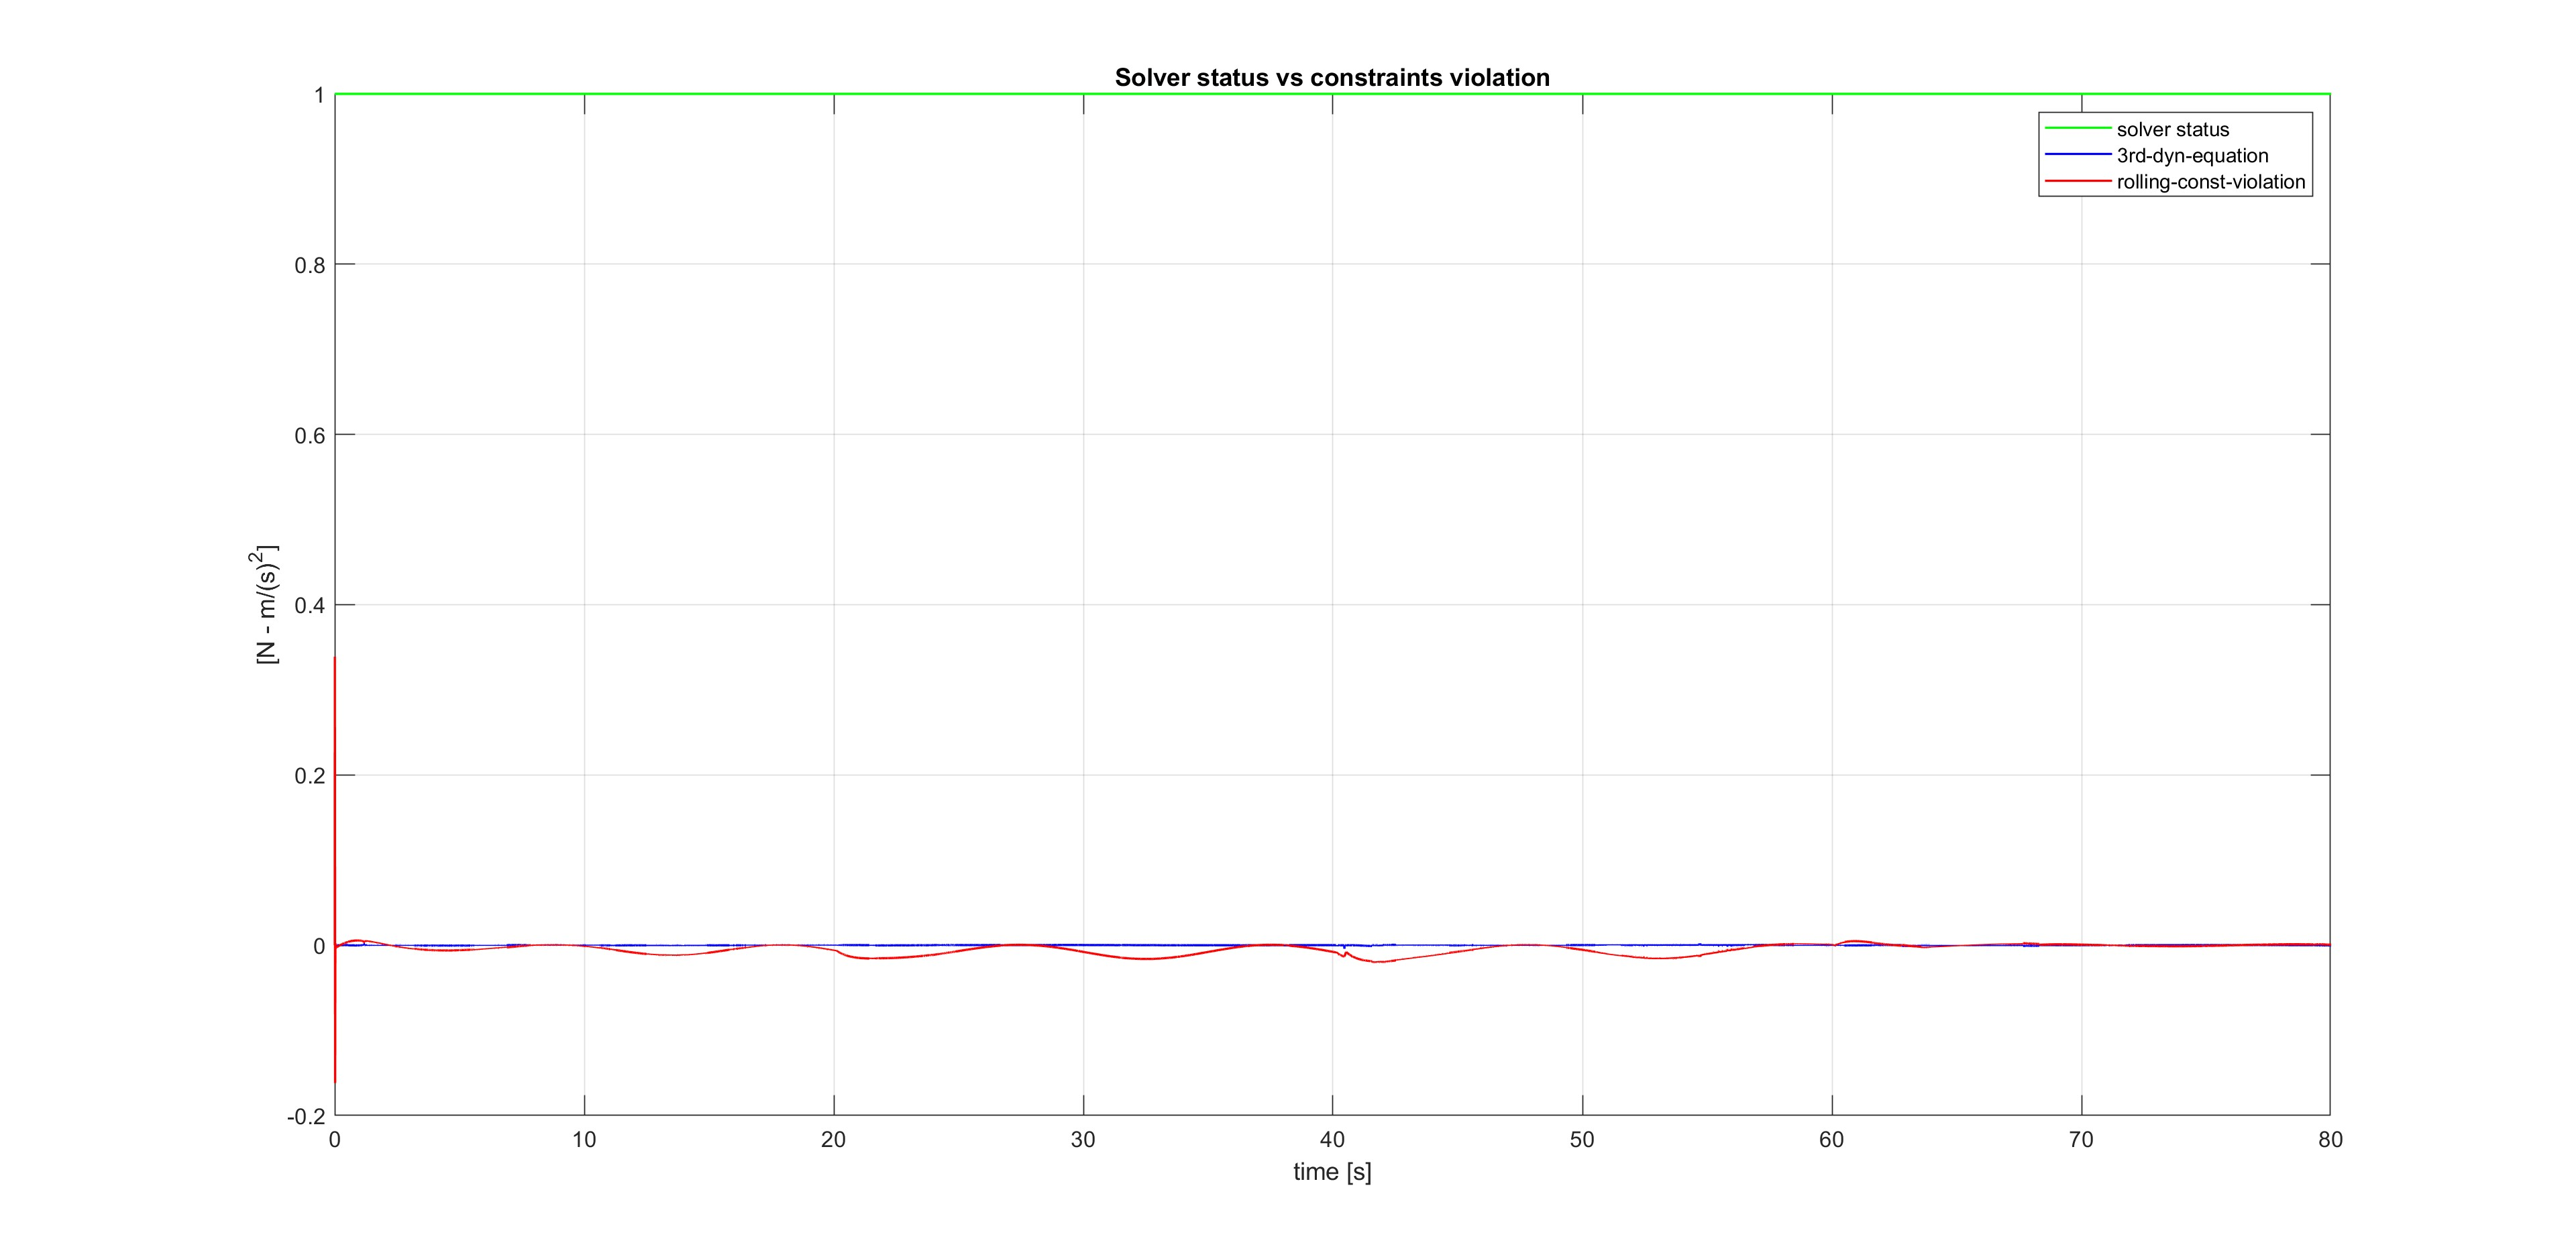
\includegraphics[width=1\linewidth]{Images/Robustness analysis/Unloaded/sinusoidal trajectory/Slipping_velocity.jpg}
    \caption{Sinusoidal trajectory slipping velocity with disturbances in the unloaded case.}
    \label{fig:Sinusoidal trajectory slipping velocity with disturbances in the unloaded case}
\end{figure}


\subsection{Sinusoidal Trajectory in the case of half load}
\label{subsec:Sinusoidal Trajectory in the case of half load}

Figures \ref{fig:Sinusoidal trajectory position error with disturbances in the case of half load} and \ref{fig:Sinusoidal trajectory velocity error with disturbances in the case of half load}, show the nominal and actual trajectories in position and velocity respectively for the condition of half load, and also in this case, after the transient, the actual trajectories approach the nominal ones.
Also in this case, some overshoots appear in Figure \ref{fig:Sinusoidal trajectory velocity error with disturbances in the case of half load} due to the discontinuous acceleration profile.

\begin{figure}
    \centering
    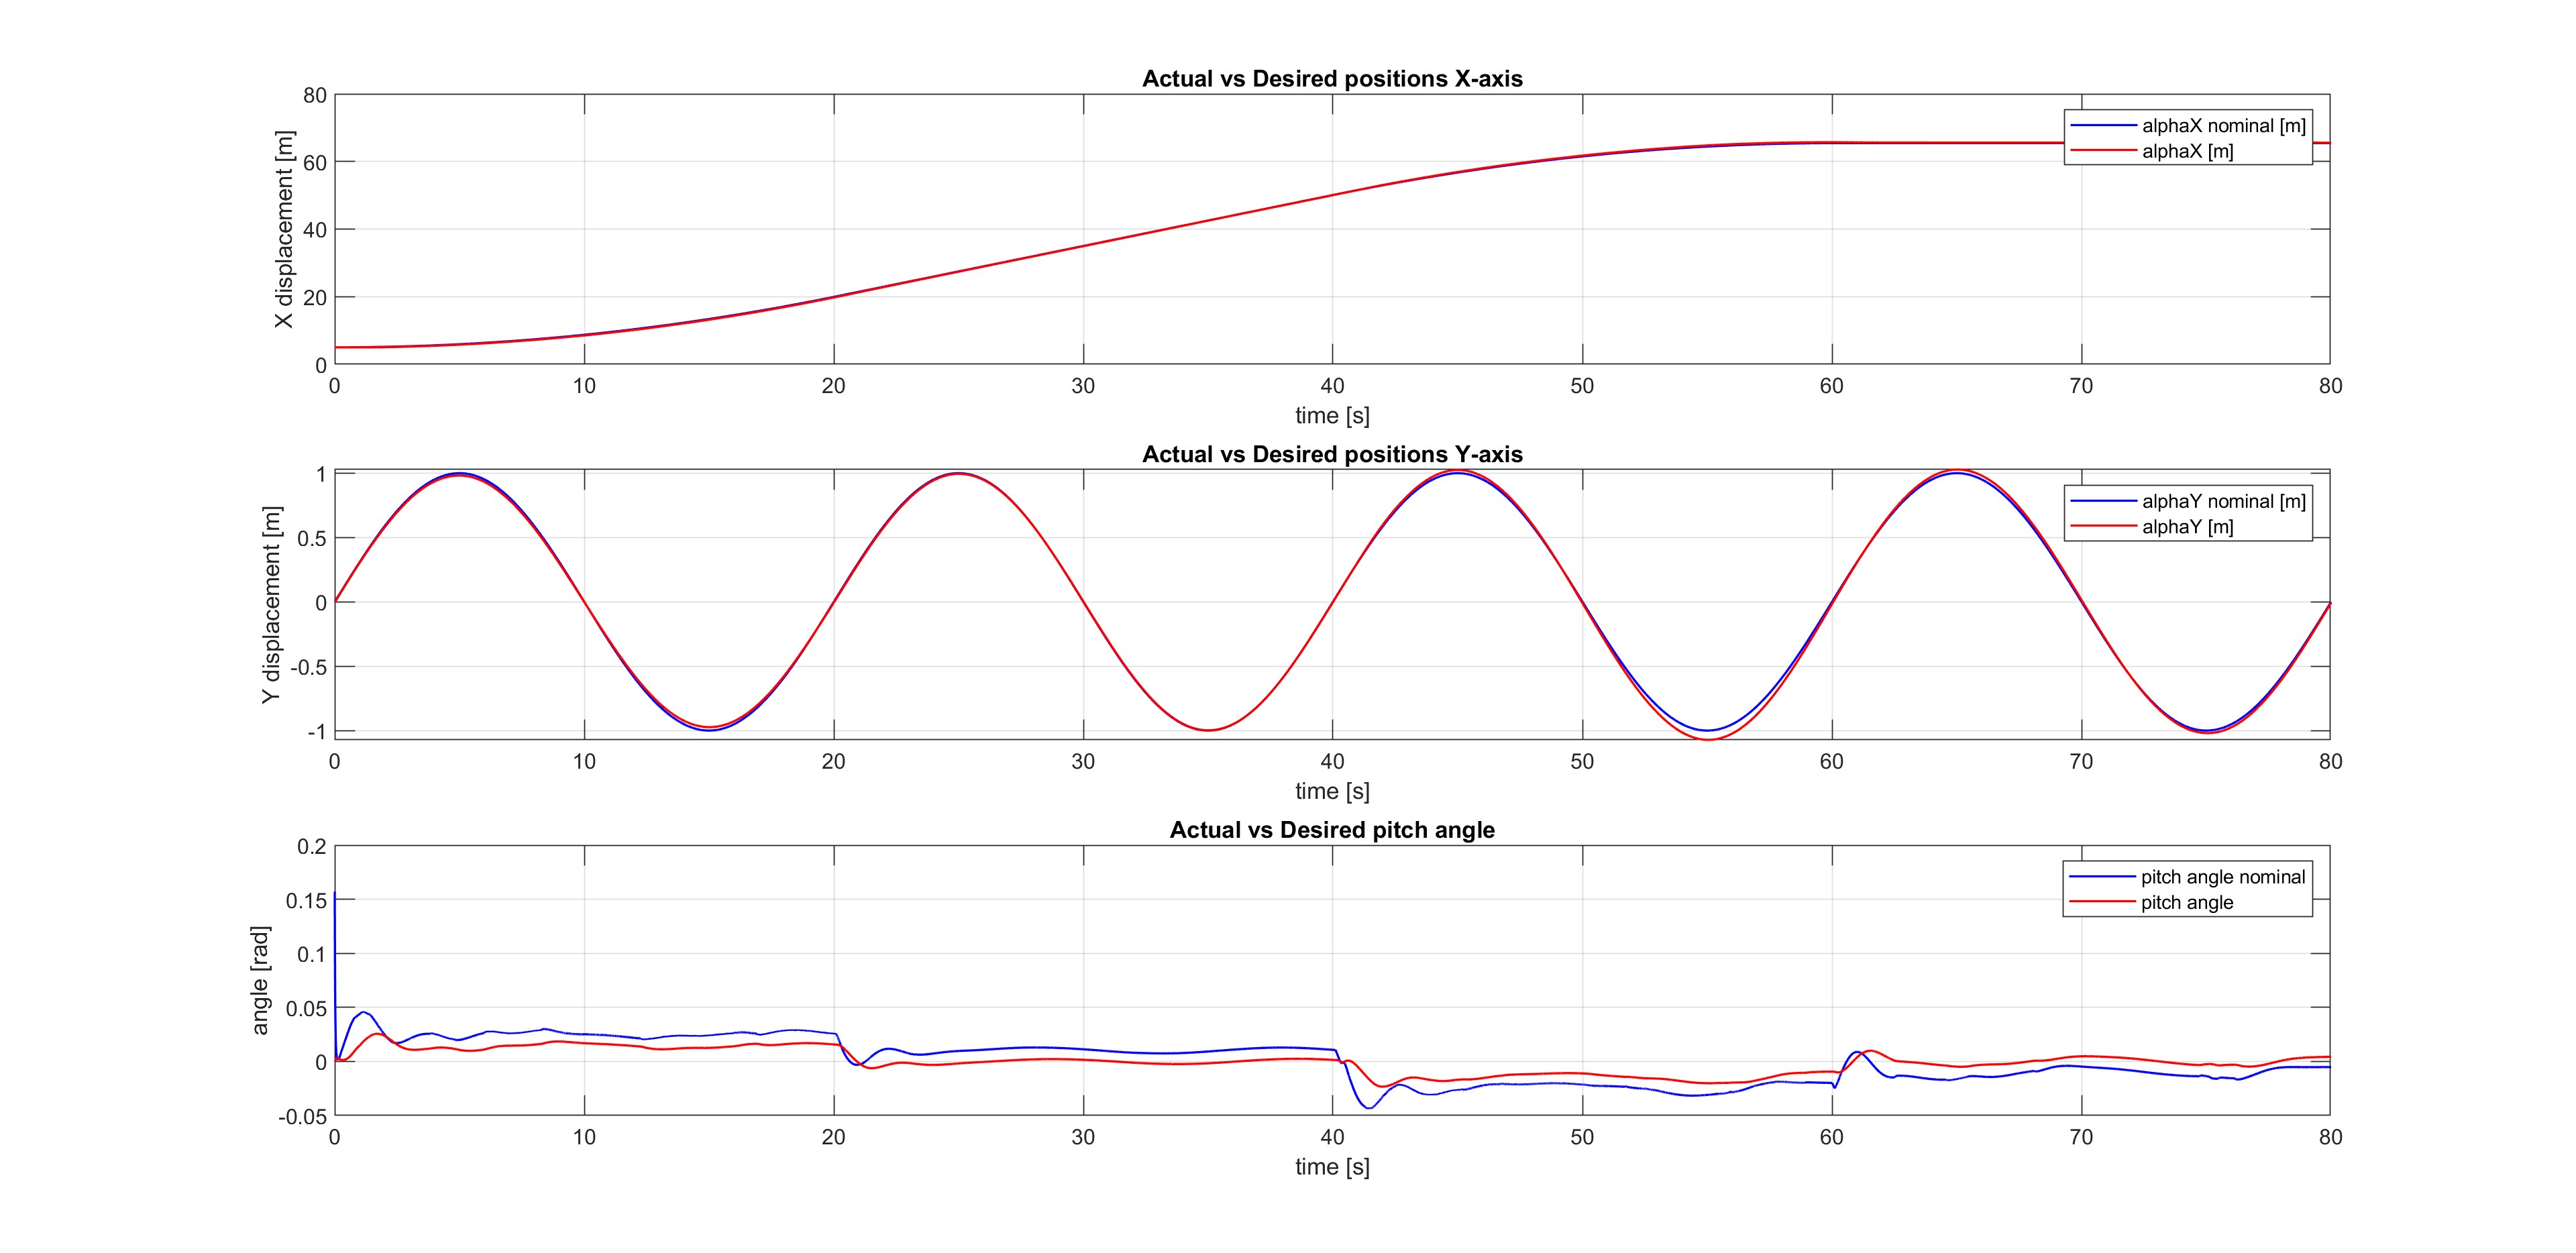
\includegraphics[width=1\linewidth]{Images/Robustness analysis/intermediate load/sinusoidal trajectory/Position_error.jpg}
    \caption{Sinusoidal trajectory position error with disturbances in the case of half load.}
    \label{fig:Sinusoidal trajectory position error with disturbances in the case of half load}
\end{figure}

\begin{figure}
    \centering
    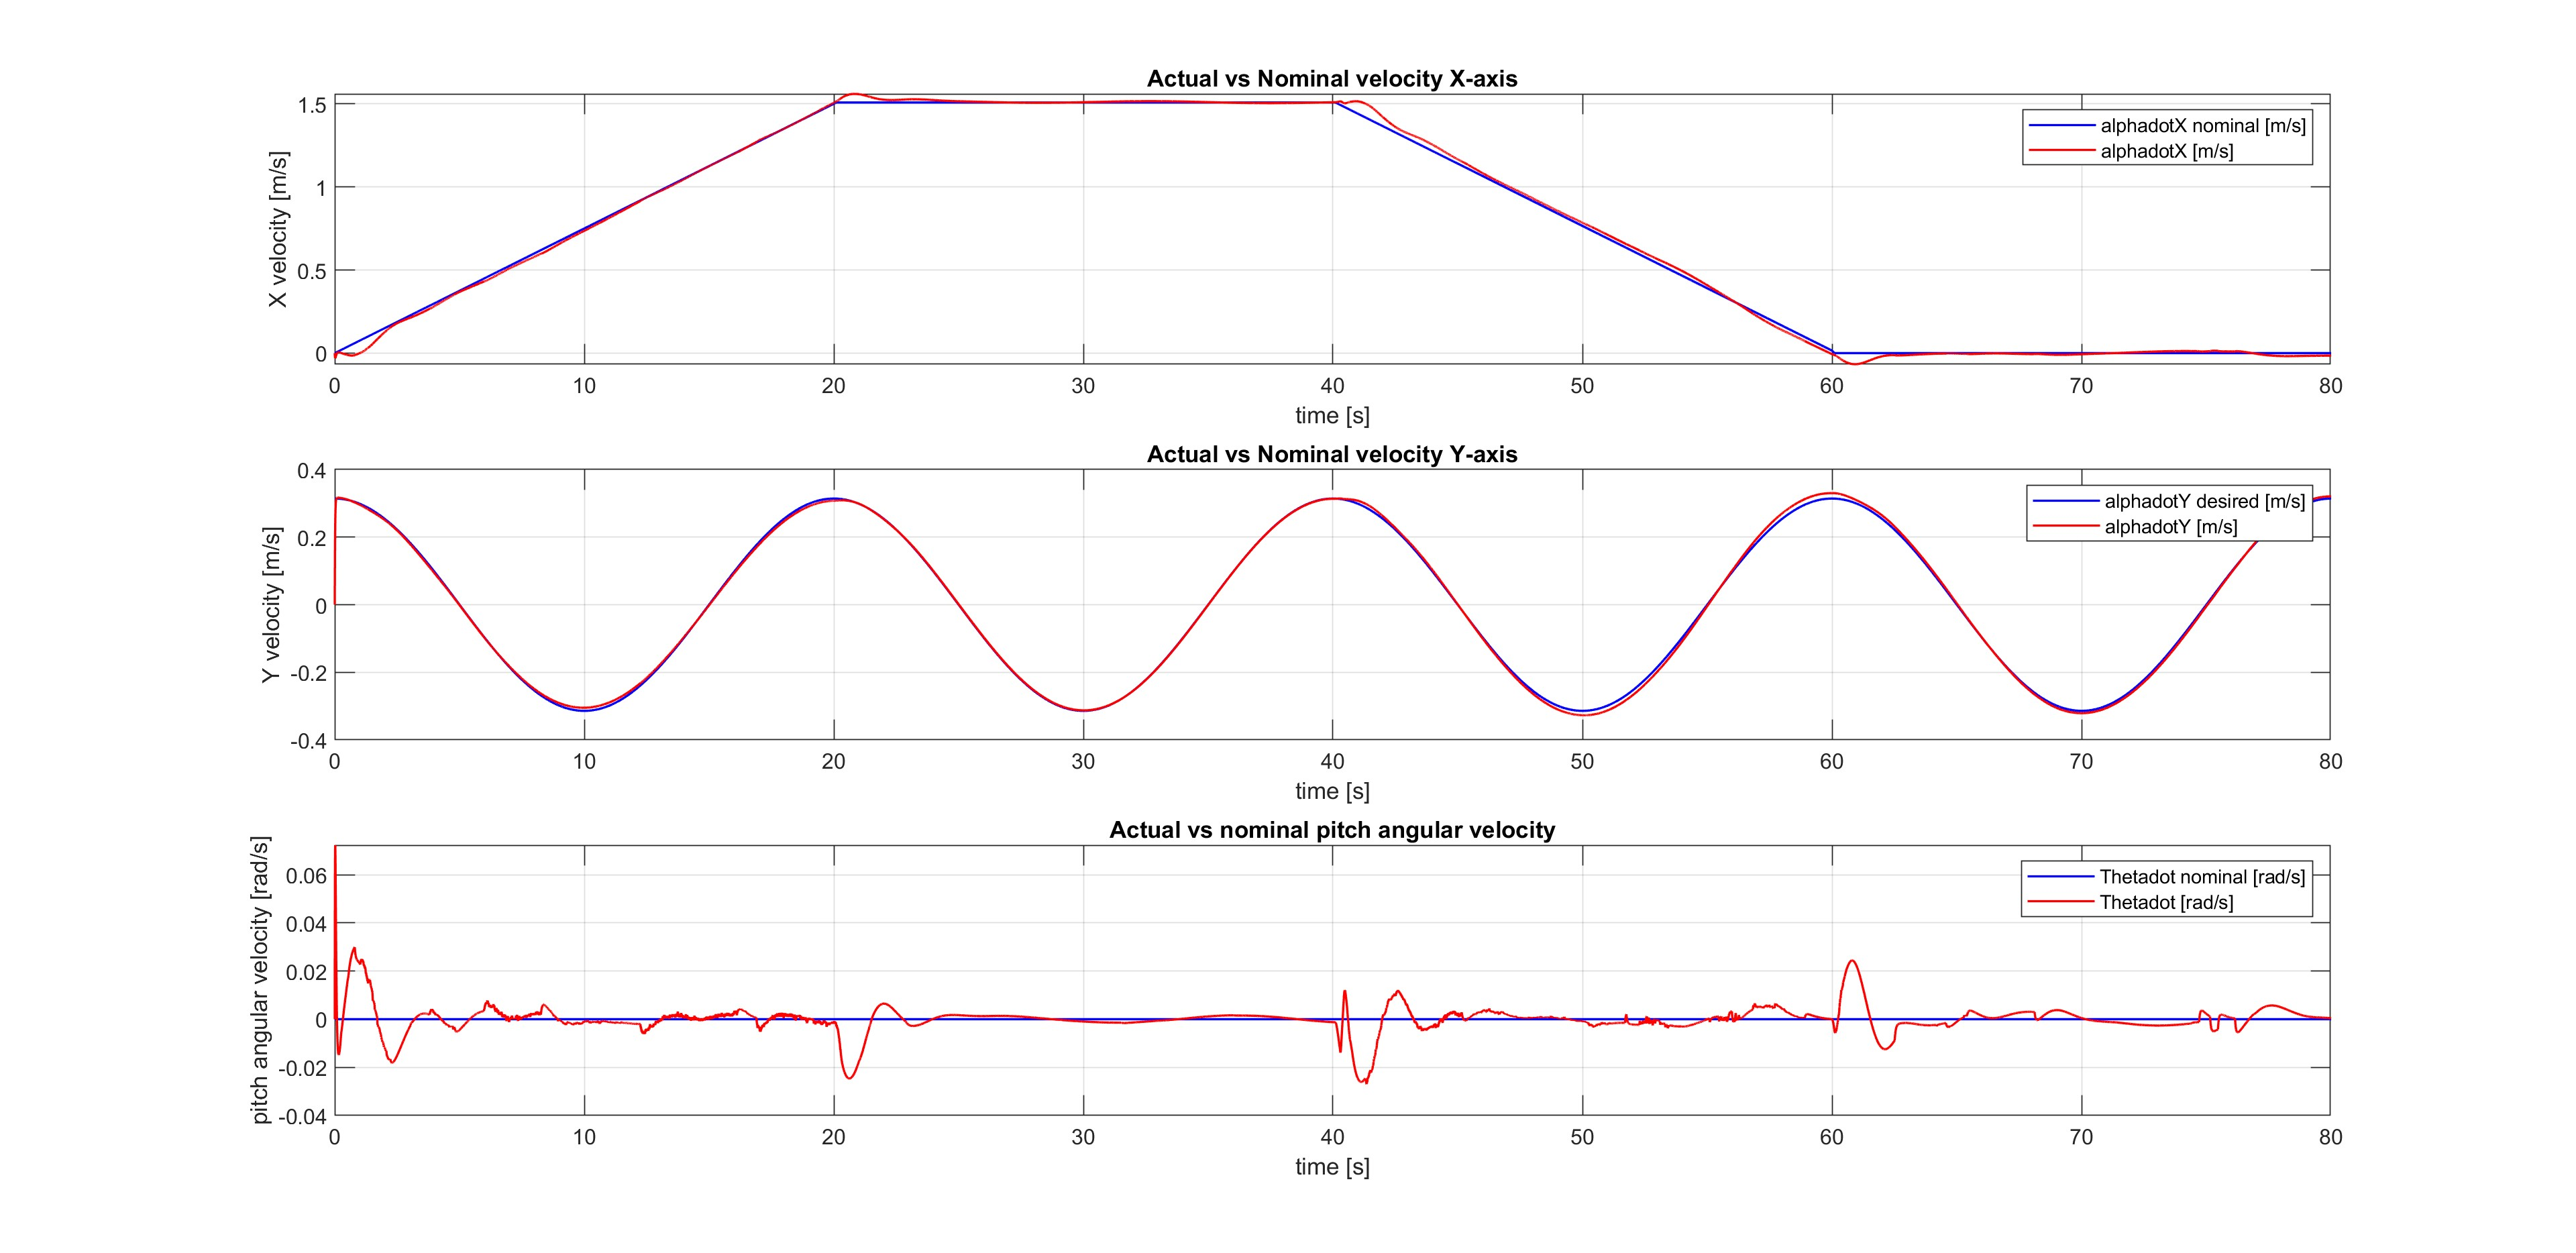
\includegraphics[width=1\linewidth]{Images/Robustness analysis/intermediate load/sinusoidal trajectory/Velocity_error.jpg}
    \caption{Sinusoidal trajectory velocity error with disturbances in the case of half load.}
    \label{fig:Sinusoidal trajectory velocity error with disturbances in the case of half load}
\end{figure}

Figure \ref{fig:Sinusoidal trajectory slipping velocity with disturbances in the case of half load} instead shows in red the slipping velocity between the wheels and the terrain which is almost zero, and in green the solver status which is always =1.

\begin{figure}
    \centering
    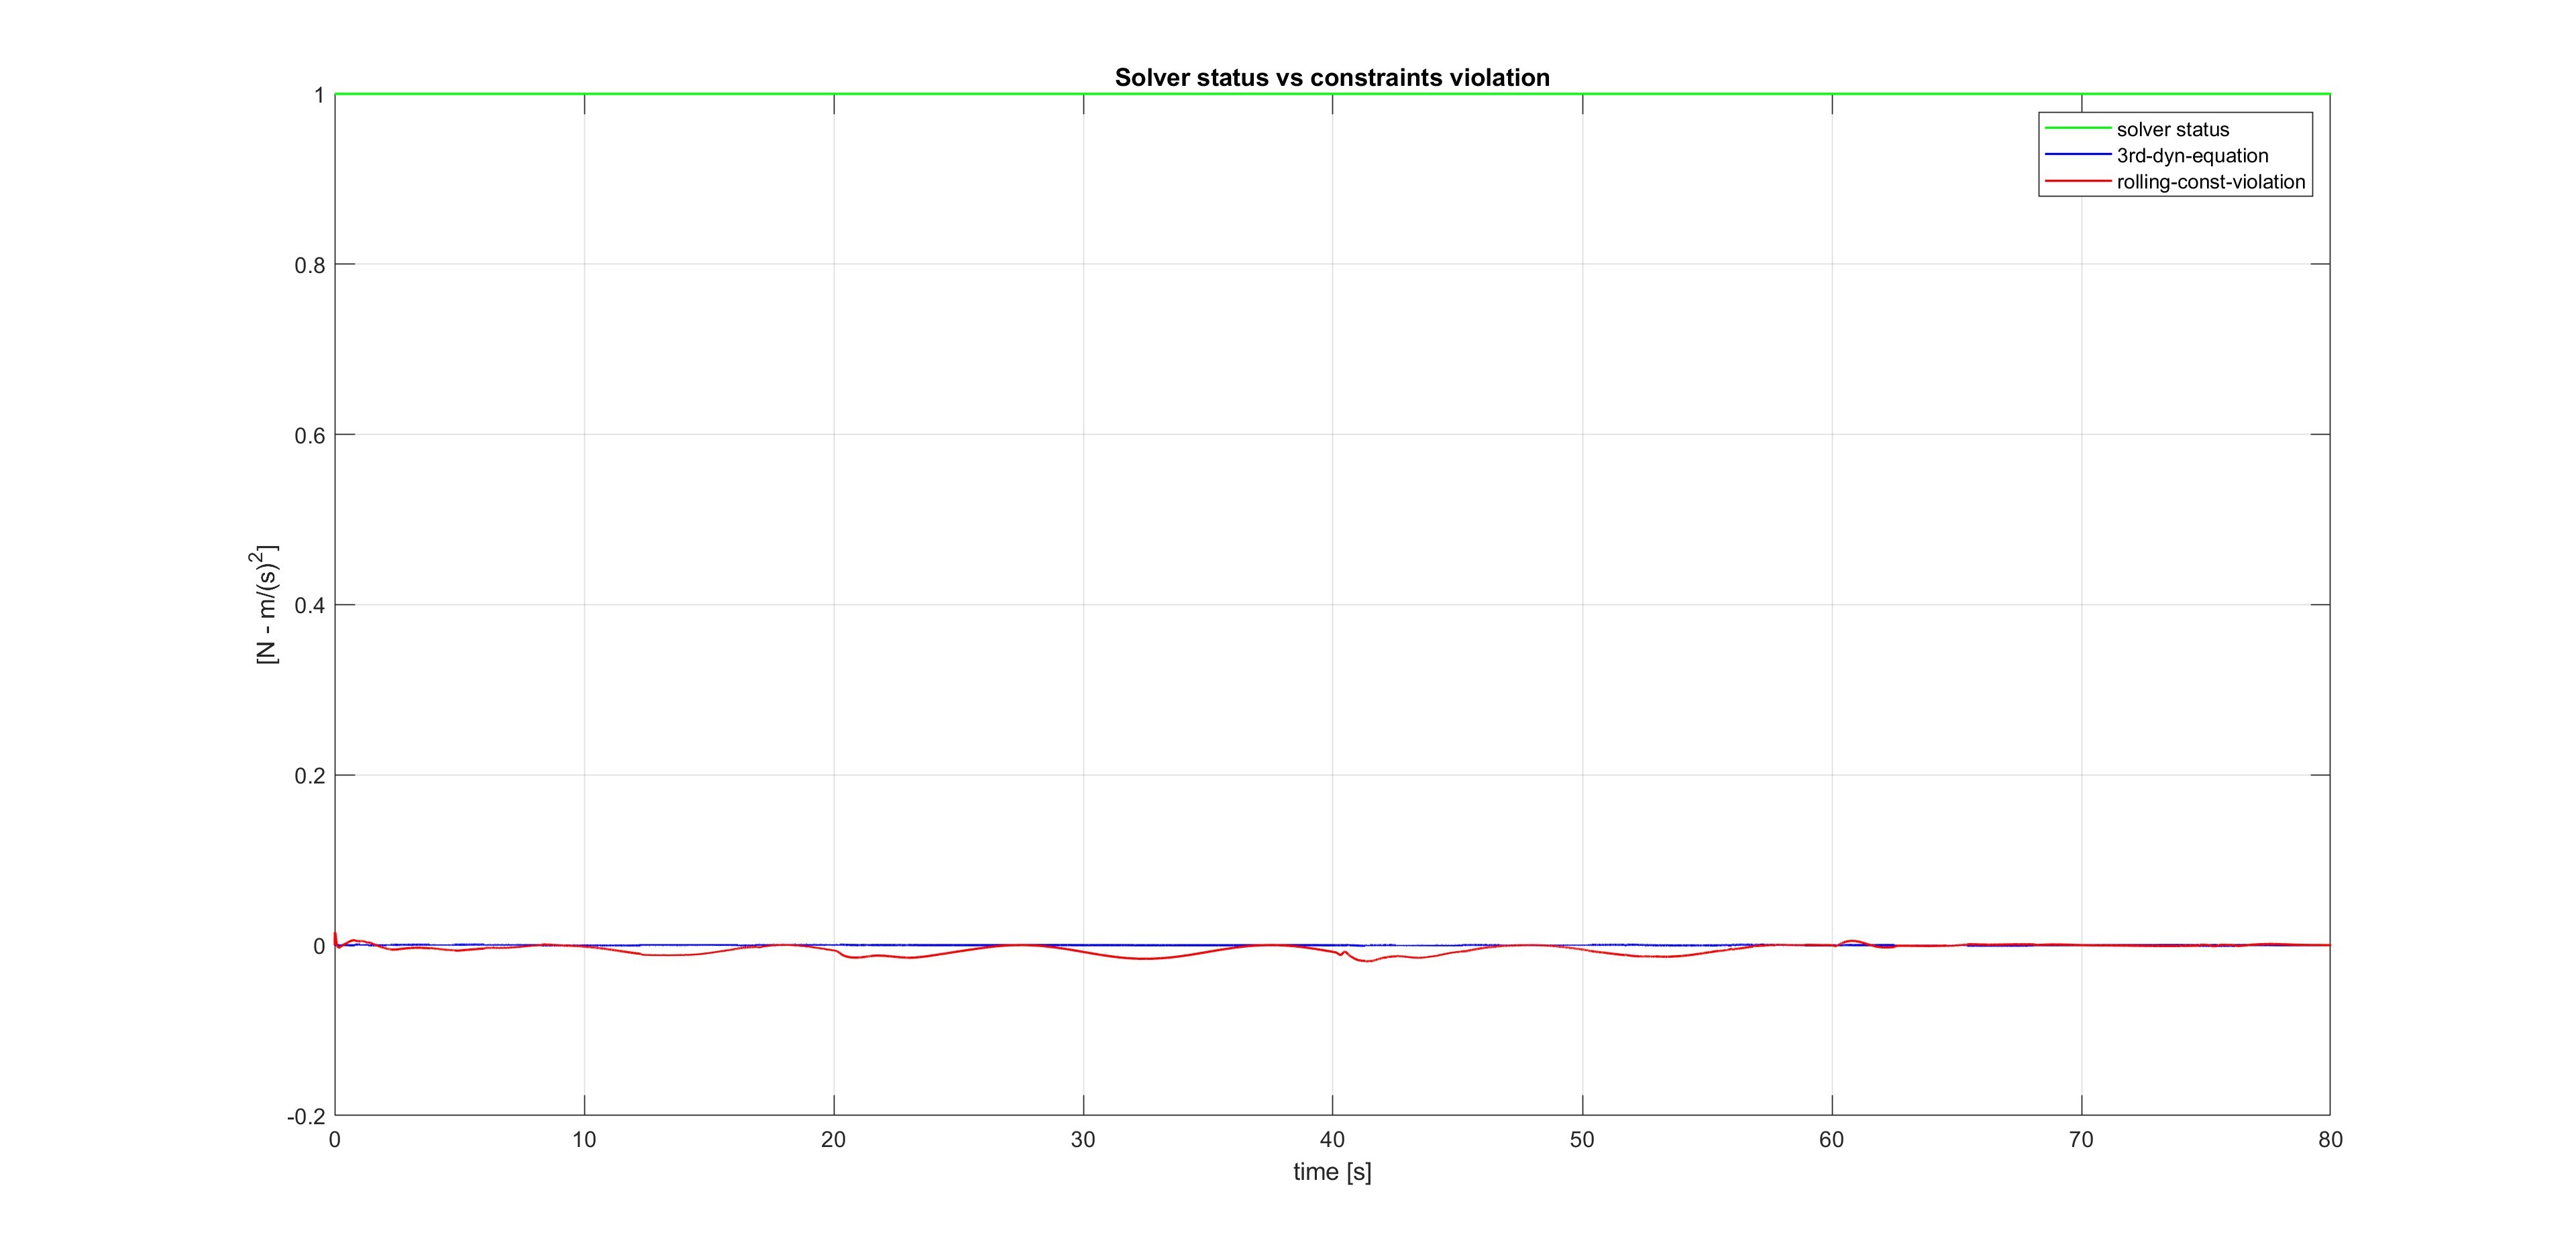
\includegraphics[width=1\linewidth]{Images/Robustness analysis/intermediate load/sinusoidal trajectory/Slipping_velocity.jpg}
    \caption{Sinusoidal trajectory slipping velocity with disturbances in the case of half load.}
    \label{fig:Sinusoidal trajectory slipping velocity with disturbances in the case of half load}
\end{figure}

\subsection{Sinusoidal Trajectory in the case of maximum load}
\label{subsec:Sinusoidal Trajectory in the case of maximum load}

Figures \ref{fig:Sinusoidal trajectory position error with disturbances in the case of maximum load} and \ref{fig:Sinusoidal trajectory velocity error with disturbances in the case of maximum load}, show the nominal and actual trajectories in position and velocity respectively for the worse case scenario in which the E-Cargo is loaded at its maximum capacity.
Also in this last case some overshoots can be noticed in Figure \ref{fig:Sinusoidal trajectory velocity error with disturbances in the unloaded case} due to the discontinuous acceleration profile.

\begin{figure}
    \centering
    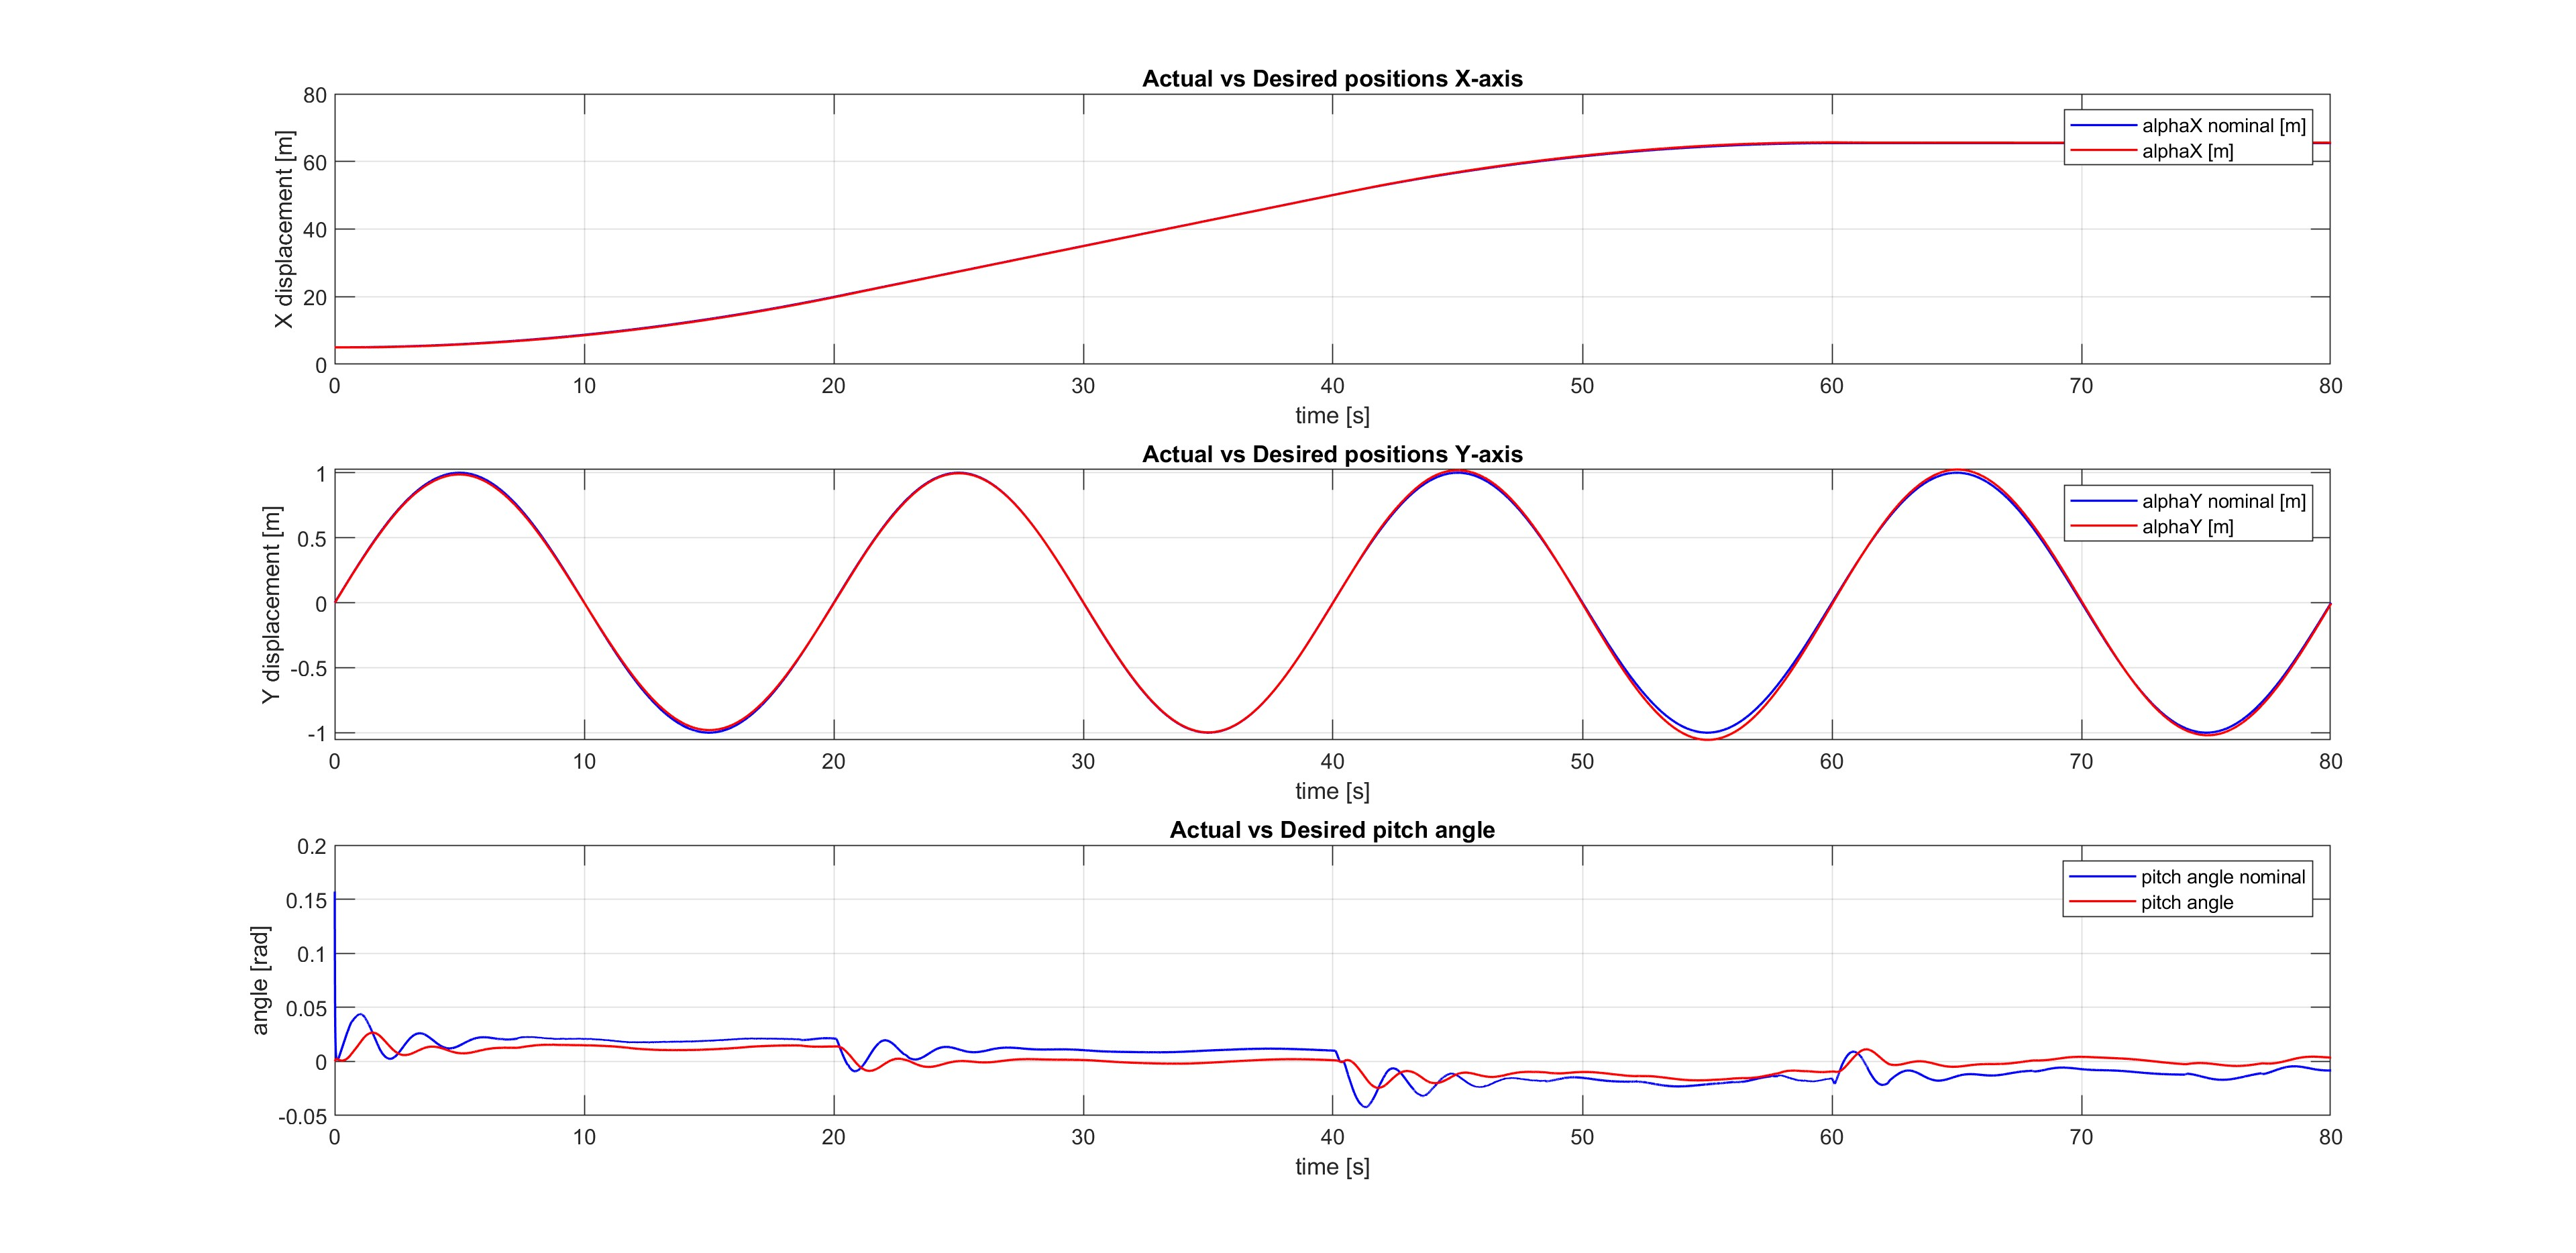
\includegraphics[width=1\linewidth]{Images/Robustness analysis/maximum load/sinusoidal trajectory/Position_error.jpg}
    \caption{Sinusoidal trajectory position error with disturbances in the case of maximum load.}
    \label{fig:Sinusoidal trajectory position error with disturbances in the case of maximum load}
\end{figure}

\begin{figure}
    \centering
    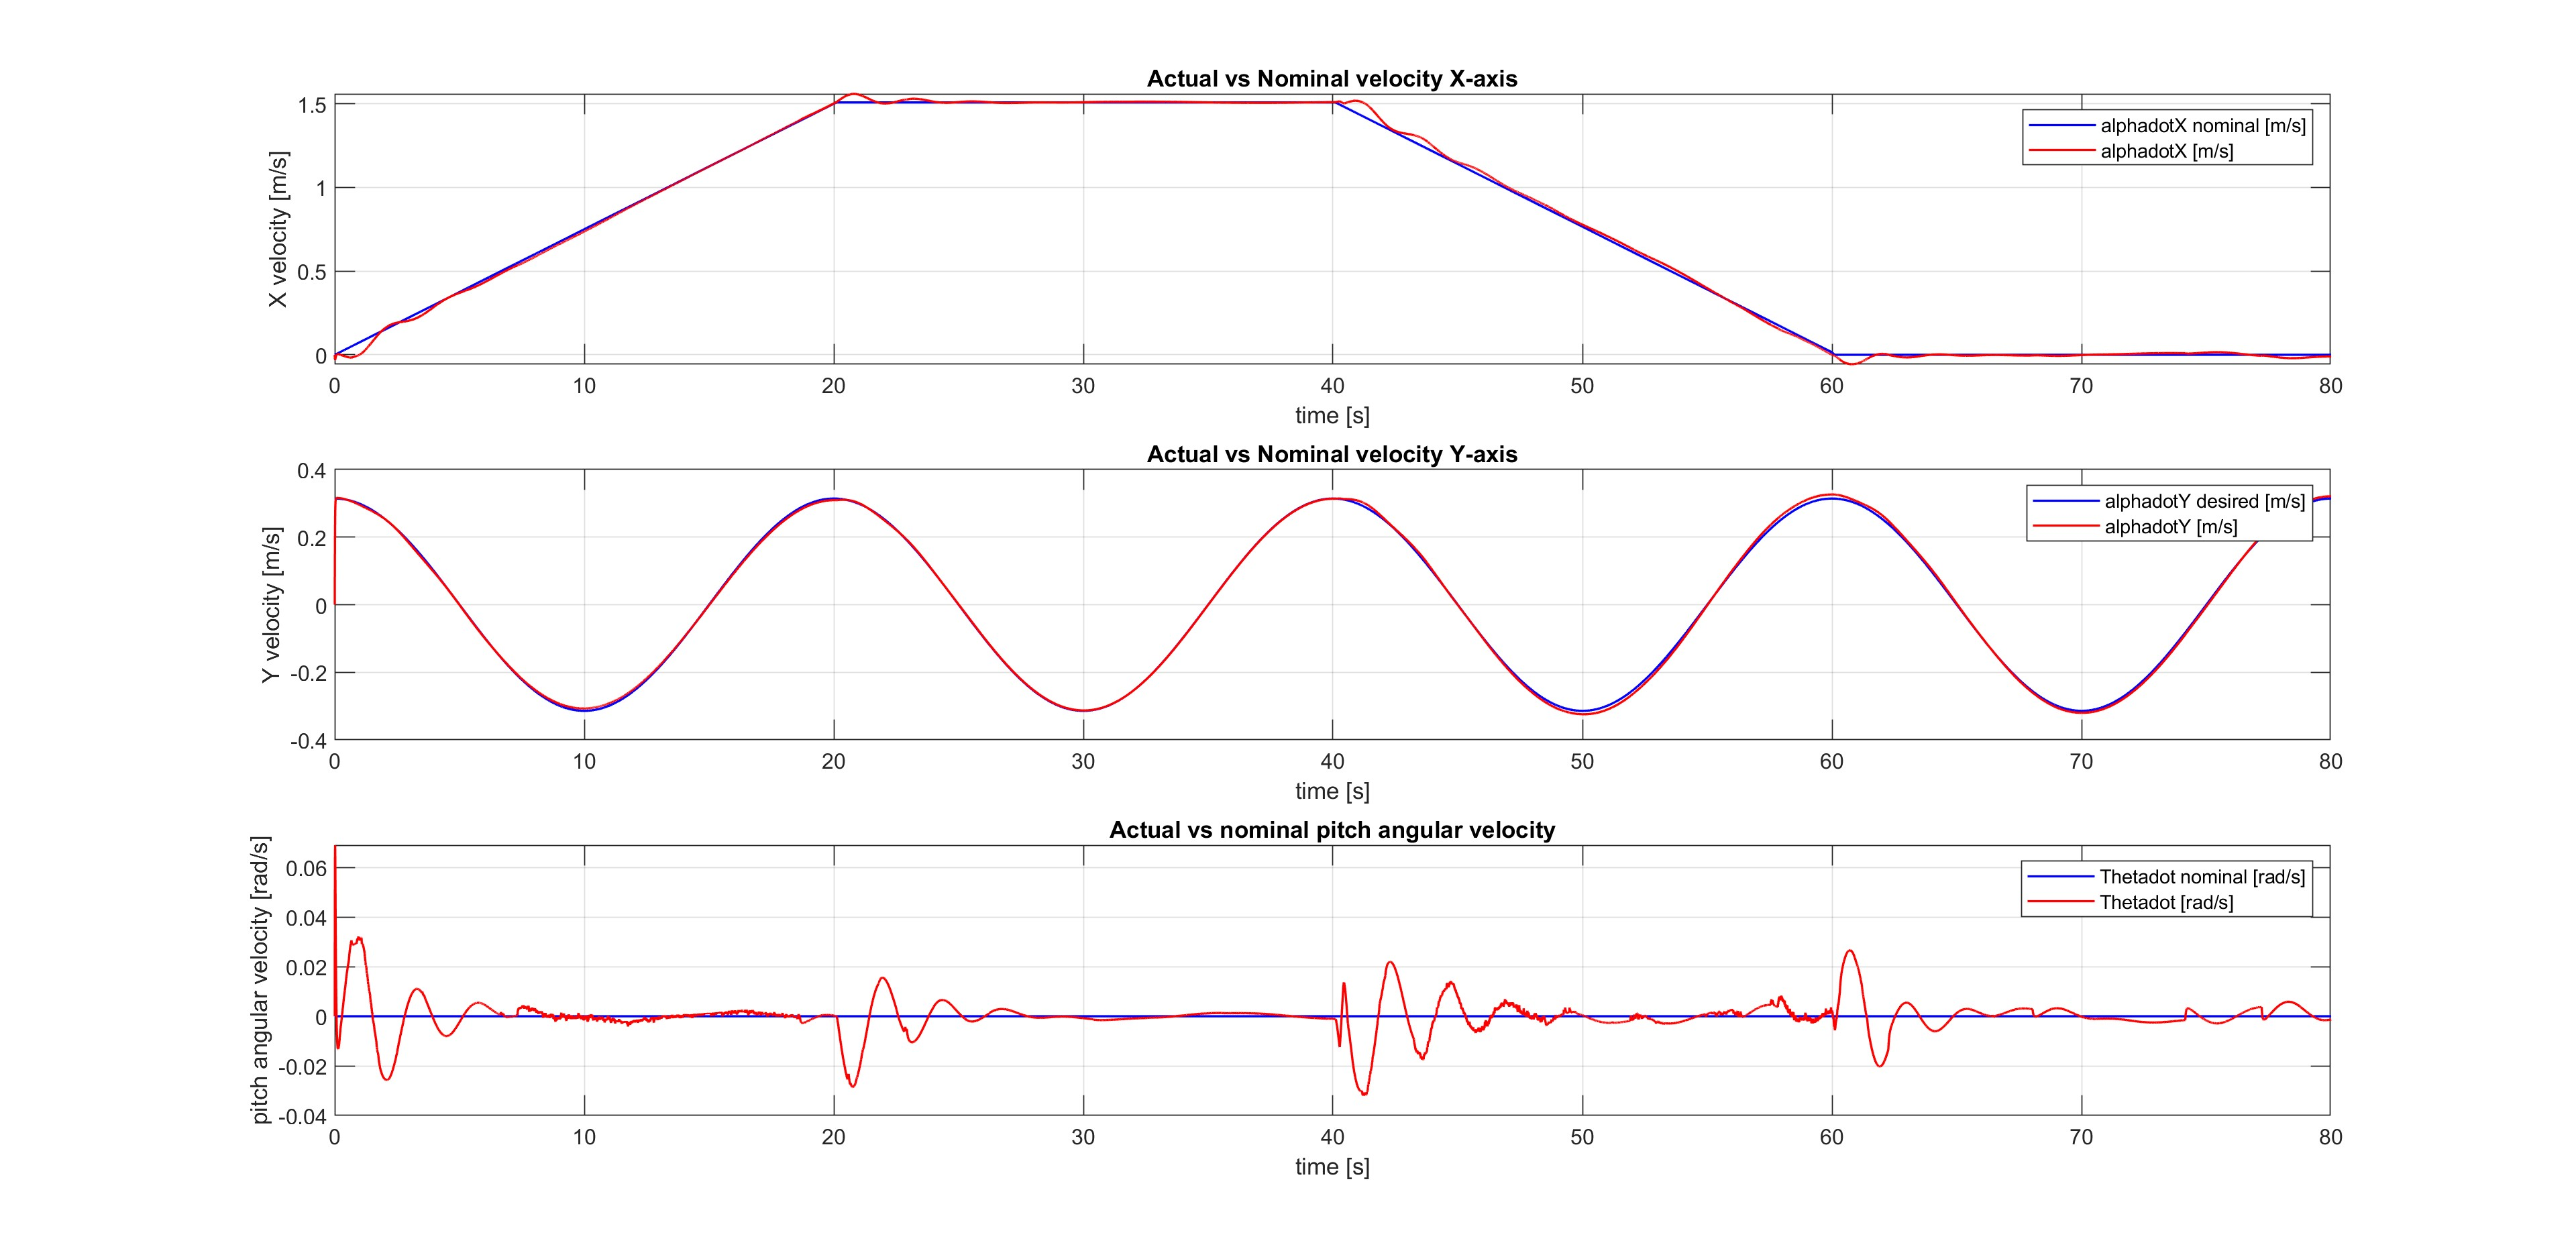
\includegraphics[width=1\linewidth]{Images/Robustness analysis/maximum load/sinusoidal trajectory/Velocity_error.jpg}
    \caption{Sinusoidal trajectory velocity error with disturbances in the case of maximum load.}
    \label{fig:Sinusoidal trajectory velocity error with disturbances in the case of maximum load}
\end{figure}

\begin{figure}
    \centering
    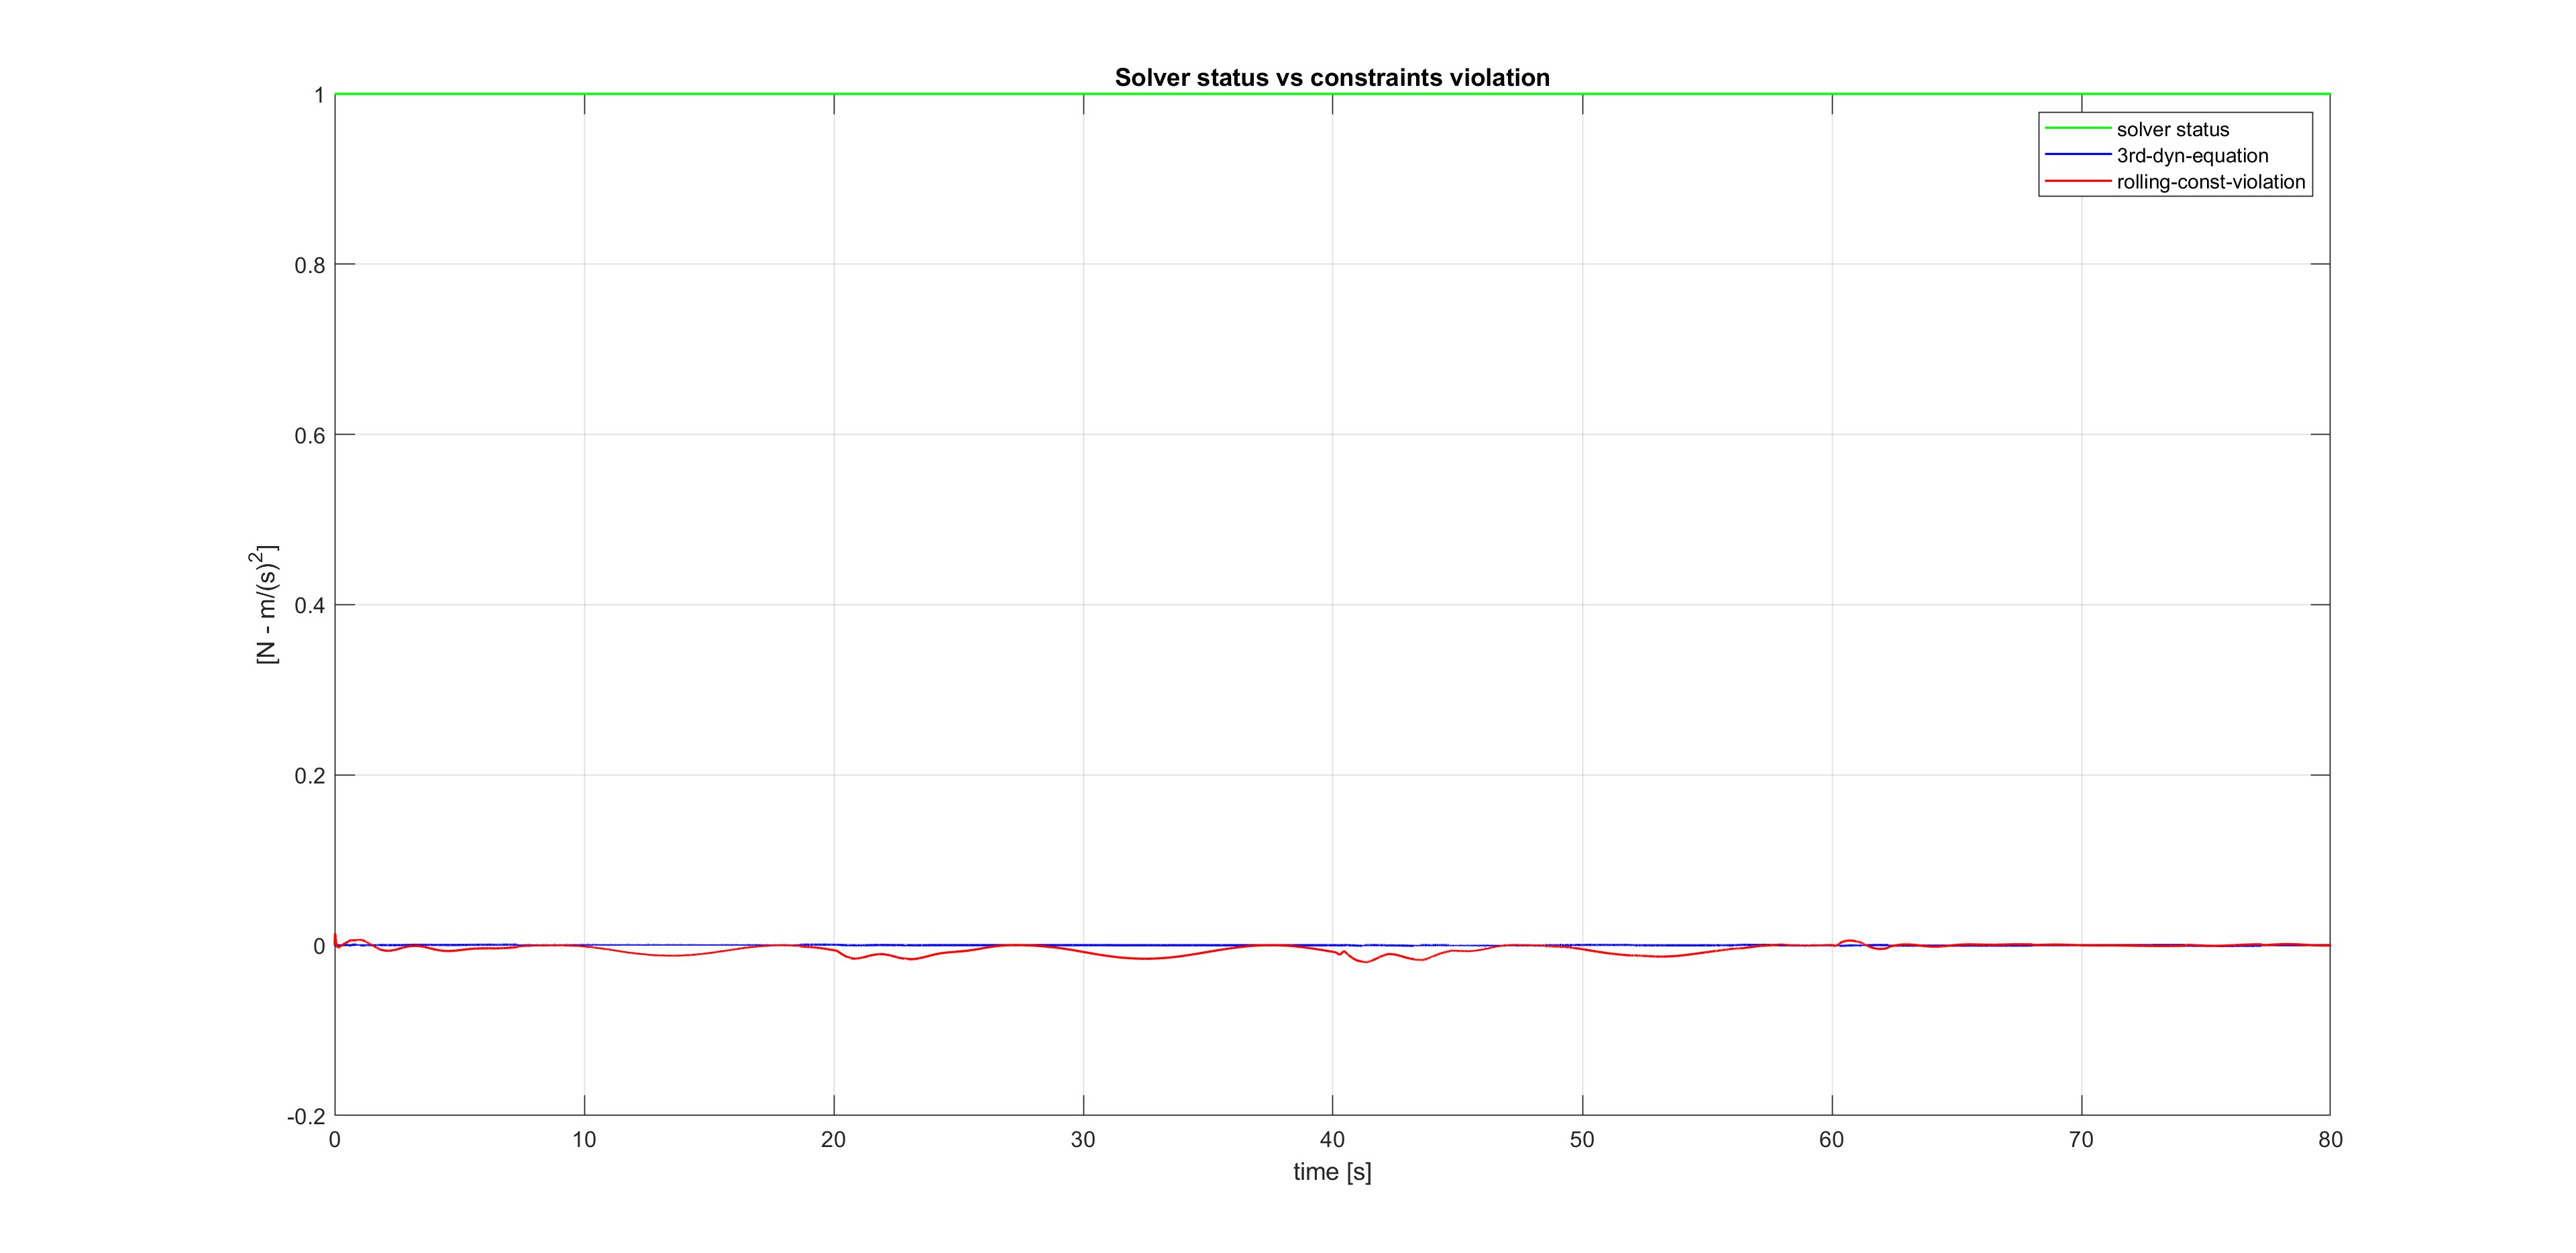
\includegraphics[width=1\linewidth]{Images/Robustness analysis/maximum load/sinusoidal trajectory/Slipping_velocity.jpg}
    \caption{Sinusoidal trajectory slipping velocity with disturbances in the case of maximum load.}
    \label{fig:Sinusoidal trajectory slipping velocity with disturbances in the case of maximum load}
\end{figure}

Figure \ref{fig:Sinusoidal trajectory slipping velocity with disturbances in the case of maximum load} instead shows how the solver never fails to provide a solution respecting the constraints.